%\documentclass[12pt,a4paper]{report}
\documentclass[12pt,a4paper,oneside,onecolumn,openright]{book}
% set the document language
\usepackage[italian]{babel}
% set the encoding used by your editor here (default is utf8)
\usepackage[utf8]{inputenc}
\usepackage[T1]{fontenc}

% math packages
\usepackage{amsmath}
\usepackage{amssymb}
\usepackage{lmodern}
% page margins settings
\usepackage[inner=3cm,outer=2.5cm,top=3cm,bottom=2.5cm]{geometry}
%\usepackage{indentfirst}

% other packages
\usepackage{array}
\usepackage{enumitem}
\usepackage{subfigure}
\usepackage{graphicx}
\usepackage{verbatim}
\usepackage{listings}
\usepackage{url}
\usepackage[hidelinks]{hyperref}
\usepackage[export]{adjustbox}
\usepackage{latexsym}
\usepackage{tabularx}
\usepackage{ragged2e}
\usepackage{mathtools}
\DeclarePairedDelimiter\floor{\lfloor}{\rfloor}
\DeclarePairedDelimiter\ceil{\lceil}{\rceil}
% \usepackage{Mathematics}
% custom colors
\usepackage{color}
\usepackage{wrapfig}
\usepackage{gensymb}
\usepackage{caption}
\usepackage{tikz}
\usepackage{forest}
\usepackage{tikz-qtree}

\usetikzlibrary{shadows}
\definecolor{light-gray}{gray}{0.96}
\definecolor{cyan}{RGB}{230,230,255}
\definecolor{dkgreen}{rgb}{0,0.6,0}
\definecolor{gray}{rgb}{0.5,0.5,0.5}
\definecolor{mauve}{rgb}{0.58,0,0.82}
\definecolor{iceberg}{rgb}{0.44, 0.65, 0.82}
% \definecolor{blue}{RGB}{44, 44, 210}

\hypersetup{
colorlinks=true,
linkcolor=black,
% filecolor=blue,
urlcolor=blue,
% pdftitle={Overleaf Example},
}

\urlstyle{same}
\graphicspath{ {./images/} }

% environment for bash code
\lstset{ %
  language=bash,                % the language of the code
  basicstyle=\footnotesize,           % the size of the fonts that are used for the code
  numbers=left,                   % where to put the line-numbers
  numberstyle=\footnotesize,          % the size of the fonts that are used for the line-numbers
  stepnumber=1,                   % the step between two line-numbers. If it's 1, each line 
                                  % will be numbered
  numbersep=5pt,                  % how far the line-numbers are from the code
  backgroundcolor=\color{white},      % choose the background color. You must add \usepackage{color}
  showspaces=false,               % show spaces adding particular underscores
  showstringspaces=false,         % underline spaces within strings
  showtabs=false,                 % show tabs within strings adding particular underscores
%  frame=single,                   % adds a frame around the code
  rulecolor=\color{black},        % if not set, the frame-color may be changed on line-breaks within not-black text (e.g. commens (green here))
  tabsize=2,                      % sets default tabsize to 2 spaces
  captionpos=b,                   % sets the caption-position to bottom
  breaklines=true,                % sets automatic line breaking
  breakatwhitespace=false,        % sets if automatic breaks should only happen at whitespace
  title=\lstname,                   % show the filename of files included with \lstinputlisting;
                                  % also try caption instead of title
  numberstyle=\tiny\color{gray},        % line number style
  keywordstyle=\textbf,          % keyword style
  commentstyle=\color{dkgreen},       % comment style
%  stringstyle=\color{mauve},         % string literal style
  escapeinside={\%*}{*)},            % if you want to add a comment within your code
  morekeywords={*,...,insert,-}               % if you want to add more keywords to the setù
}

% environment for python code
\lstset{
	language=Python,
	breaklines=true,
	breakatwhitespace=true ,
	backgroundcolor=\color{light-gray}
}

\newcommand{\grayScale}{0.95} % Can change the gray level here
\definecolor{codeBackground}{rgb}{\grayScale ,\grayScale ,\grayScale}
\definecolor{forestGreen}{rgb}{0.13,0.55,0.13}

\lstset{
    language=C,
    backgroundcolor=\color{codeBackground},
    tabsize=4,
    showstringspaces=false,
    showtabs=false,
    showspaces=false,
    basicstyle=\ttfamily,
    identifierstyle=\ttfamily,
    keywordstyle=\color{blue},
    stringstyle=\color{red},
    commentstyle=\color{gray},
    numberstyle=\color{magenta},
    morecomment=[l][\color{forestGreen}]{\#},
    escapechar={|}, 
}
% appendices package
%\usepackage{appendix}
% set Appendix name used in the toc
%\renewcommand{\appendixtocname}{Appendice}

% interline
\linespread{1.5}
% set numbers for subsections and show them in the toc
\setcounter{tocdepth}{3} 
\setcounter{secnumdepth}{3}

% layout package, style and settings
\usepackage{fancyhdr}
\pagestyle{fancy}

\fancypagestyle{mainmatter}{%		
		\fancyhf{} 
		\fancyhead{}
		\fancyhead[LE,RO]{\thepage}
		\fancyhead[LO]{\footnotesize{\leftmark}}
		\fancyhead[RE]{\footnotesize{\rightmark}}
		\fancyfoot{}
		\addtolength{\headwidth}{\marginparsep}
		\addtolength{\headheight}{2.5pt}
		\renewcommand{\headrulewidth}{0.3pt}
		\renewcommand{\footrulewidth}{0.0pt}
		}
\fancypagestyle{frontmatter}{%
		\fancyhf{} 
		\fancyhead[LE]{\footnotesize{\MakeUppercase{\thepage}}}
		\fancyhead[RO]{\footnotesize{\MakeUppercase{\thepage}}}
		\fancyhead[RE,LO]{}
		\fancyfoot{}
		\addtolength{\headwidth}{\marginparsep}
		\addtolength{\headheight}{2.5pt}
		\renewcommand{\headrulewidth}{0.0pt}
		\renewcommand{\footrulewidth}{0.0pt}
		}
		
		
\usepackage{fancyhdr}
\pagestyle{fancy}
		\fancyhf{} 
		\fancyhead{}
		\fancyhead[LE,RO]{\thepage} 
		\fancyhead[LO]{\footnotesize{\leftmark}}
		\fancyhead[RE]{\footnotesize{\rightmark}}
		\fancyfoot{}
		\addtolength{\headwidth}{\marginparsep}
		\addtolength{\headheight}{2.5pt}
		\renewcommand{\headrulewidth}{0.3pt}
		\renewcommand{\footrulewidth}{0.0pt}

% empty pages have no numbers
\makeatletter
\def\cleardoublepage{\clearpage\if@twoside \ifodd\c@page\else
\hbox{}
  %Potresti voler togliere il commento dalla linea seguente
  %Questa pagina � stata lasciata intenzionalmente vuota.
\thispagestyle{empty}
\newpage
\if@twocolumn\hbox{}\newpage\fi\fi\fi}
\makeatother
%????
%\textwidth=450pt\oddsidemargin=0pt

%\makeatletter 
%  \DeclareRobustCommand*\textsubscript[1]{% 
%    \@textsubscript{\selectfont#1}} 
%  \newcommand{\@textsubscript}[1]{% 
%    {\m@th\ensuremath{_{\mbox{\fontsize\sf@size\z@#1}}}}} 
\makeatother 

\begin{document}
\begin{titlepage}
\begin{center}
{
    \large
    \textbf{Università  degli studi di Modena e Reggio Emilia} \\
   	\textbf{Dipartimento di Ingegneria Enzo Ferrari} \\
    \vspace{\stretch{0.5}}
    \hspace*{0cm} \hrulefill \hspace*{0cm} \\
    \vspace{\stretch{0.5}}    
	  \vspace{\stretch{12}}
  
  
 		\huge{\bf Algoritmi di Crittografia }}\\
		\vspace{3mm}
		
		\vspace{\stretch{6}}
		\end{center}
		
\vspace{40mm}
\par
\noindent
\vspace{20mm}
\begin{center}
\hspace*{0cm} \hrulefill \hspace*{0cm} \\
{\large{\bf 
Anno Accademico 2023/24}}
\end{center}

\end{titlepage}

\pagestyle{frontmatter}
\frontmatter

% PAGINA VUOTA
%\clearpage\null\thispagestyle{empty}\clearpage
\setcounter{tocdepth}{2}
\tableofcontents

\setlength{\parindent}{12pt}
\setlength{\parskip}{1ex plus 0.5ex minus 0.2ex}
\mainmatter
\pagestyle{mainmatter}

\chapter{Introduction}

\section{Structure and Content}
\begin{itemize}

    \item \textbf{Module 1}: 
    \begin{enumerate}
        \item \textbf{\textit{intra-vehicles communications}}: nodes, sensors, ECU
        \item \textbf{\textit{signal busses}}: CAN, LIN, FlexRay, MOST, Ethernet [ T1/T1S]
        \item \textbf{\textit{car domain and OS}}
    \end{enumerate}
    
    \item \textbf{Module 2}:
    \begin{enumerate}
        \item \textbf{\textit{inter-vehicles communications}}: \textit{V2V} and \textit{V2X} (car is a node)
        \item \textbf{\textit{wireless technologies}}: Bluetooth, LoRa, C-V2X, IEE 802.11p (bd)
        \item application, messages, broadcast, GPS
    \end{enumerate}

\end{itemize}
Different \textbf{domain} or \textbf{application} needs different \textit{communications protocols}, is important to understand how each nodes in domain communicate each other (inside the car).

\newpage
\section{Intra-Vehicles}
From the 80's, where the car's control unit are isolated an there was a dedicated wires connect sensors and actuators with less electronic than now, until the reach the greates goal of evolution in the automotive sector: autonomous drive. The complexity of the number of connection from each ECU's to the other, also the number of ECU's for each car, is growing. While the number of signal increase in a liner way, the connection between ECU's is growing with a quadratic complexity $O(n^2)$.

If we examine the evolutions of the ECUs number inside an ``Audi A6'' we can observe that in 1997 it has 5 ECUs and in the 2007 it has 50 ECUs, instead the ``Tesla M3'' in the 2017 has 70 ECUs. The quadratic increase of ECUs number, however has reach a cap for two main reason: the cost and the space inside the car. Traditionally one ECUs is responsible of one task, but nowadays it could be two type of trends:
\begin{enumerate}[nosep]
    \item \textit{distributed of function across ECUs}
    \item \textit{integration of multiple function in one ECU}
\end{enumerate}

\section{Architectures}

\begin{figure}[h]
    \centering
    \begin{minipage}[t]{0.45\textwidth}
        \centering
        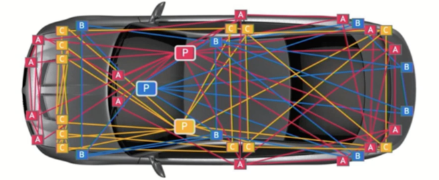
\includegraphics[width=\textwidth]{img/domain_architecture}
        \caption{\textit{Domain Architecture}}
        
        \begin{flushleft}
            \begin{enumerate}[nosep]
                \item central domain controller (\textbf{P}) or high performance computer
                \item ability to handle more complex functions
                \item cost optimization
                \item cable harness is rigid and expensive
            \end{enumerate}
        \end{flushleft}

    \end{minipage}
    \begin{minipage}[t]{0.45\textwidth}
        \centering
        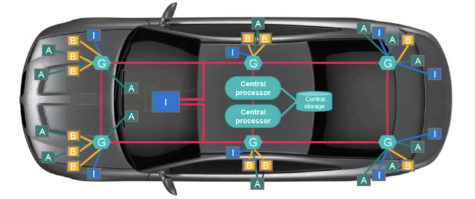
\includegraphics[width=\textwidth]{img/zonal_architecture}
        \caption{\textit{Zonal Architecture}}
        
        \begin{flushleft}
            \begin{enumerate}[nosep]
                \item local ethernet per zone (\textbf{G})
                \item ultra high-speed secured backbone between zone
                \item centralized software
                \item central computer storage
            \end{enumerate}
        \end{flushleft}
        
    \end{minipage}
\end{figure}
\chapter{Crittografia Simmetrica}

\begin{figure}[h]
    \centering
    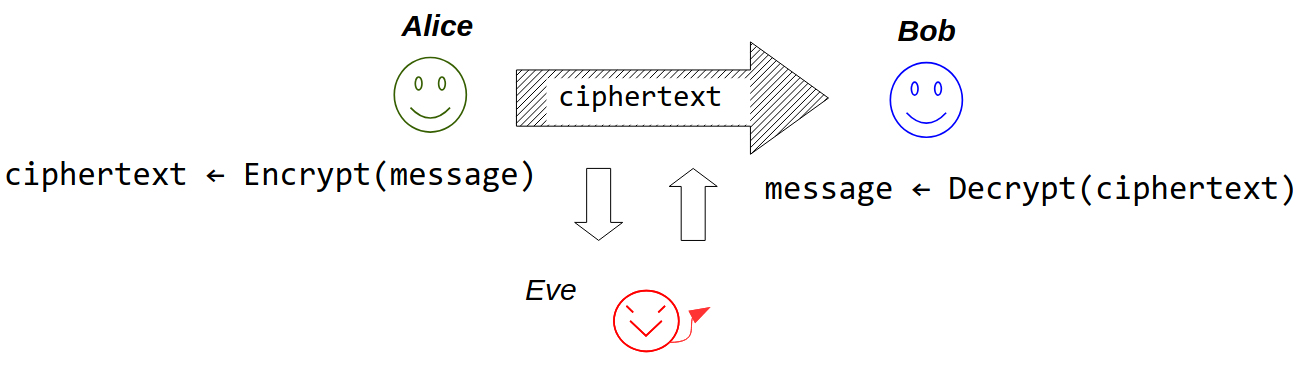
\includegraphics[width=\textwidth]{img/crypto_symm_1.png}
\end{figure}

Le garanzie di sicurezze che si cercano di mantenere sono:
\begin{itemize}[nosep]
    \item \textbf{confidenzialità}: Eve non può accedere a nessuna della informazioni sul messaggio.
    \item \textbf{autenticazione}: Bob può verificare se il messaggio non è stato inviato da Alice, viene anche chiamata \textbf{\textit{data orgin authenticity}} nel contesto della comunicazioni e implica anche la protezione contro modifiche illegittime (\textbf{integrità}).
\end{itemize}

\begin{flushleft}
    La sicurezza non esiste in natura è quindi necessario idearla e modellarla, questa prima parte prende il nome di \textit{Definitional Activity}. È comunque importante ricordare che le \textbf{definizioni} possono essere \textbf{errate} principalmente per errori nella modellazione o nello sviluppo software, ma anche perché non si è stato in grado di modellare quello che era invece richiesto. Un altro errore che si può essere portati a fare è quello di utilizzare in maniera errata certe definizioni ad esempio al di fuori del contesto per cui era stata definita. \newline
    \textbf{\textit{Definitional Activity}}: permette di descrivere che cosa l'avversario può \textbf{fare} e cosa può \textbf{vedere}. Esistono molteplici modi per definire la sicurezza in maniera più formale, uno tra questi è la \textbf{\textit{simulation-based security}} dove viene definita una funzione ideale che soddisfa la definizione di security e poi dimostrare che la funzione costruita si comporti come quella ideale.
\end{flushleft}

\begin{figure}[h]
    \centering
    \begin{large}
        \textbf{\textit{First Adversary Model}} \\
    \end{large}
    Quindi modelliamo e identifichiamo le casistiche e tipologie di un attaccante. \\

    \begin{minipage}[t]{0.50\textwidth}
        \centering
        \begin{boxA}
            \textcolor{red}{\textbf{\textit{Attack Model: Passive Eavesdropper (EAV)}}} \\
            Ha capacità di lettura dei soli \textit{ciphertext} e non è capace di \textbf{scegliere nulla}
        \end{boxA}
    \end{minipage}
    \begin{minipage}[t]{0.45\textwidth}
        \centering
        \begin{boxA}
            \textcolor{red}{\textbf{\textit{Security Goal: Indistinguishably}}} \\
            L'avversario non può distinguere il \textit{ciphertext} da sequenza di caratteri random.
        \end{boxA}
    \end{minipage}
\end{figure}

\begin{flushleft}
    Modellando in questo modo il nostro avversario è possibile osservare che non viene descritto nulla sul nascondere la lunghezza del \textit{plaintext}, infatti per questa prima modellazione l'avversario può vedere la lunghezza del \textit{plaintext}. \\
    \textbf{Nota}: la crittografia non ha come obiettivo quello di nascondere la lunghezza del testo in chiaro, nel caso in cui questa informazione fosse confidenziale, è necessario proteggerla a livello applicativo.
\end{flushleft}

\begin{flushleft}
    Le capacità di un avversario vengono espresse e descritte tramite degli algoritmi chiamati \textbf{esperimenti}, che vengono eseguiti da un'entità chiamata \textbf{\textit{challenger}} (che per semplicità andiamo ad identificare nell'attore onesto). \\
    Come prima andiamo ad analizzare \textbf{\textit{IND-EAV}}, il \textit{challenger} va a scegliere un messaggio \textbf{m} che viene scelto con la stessa probabilità tra:
    \begin{itemize}[nosep]
        \item dati random: $m \leftarrow \{0, 1\}^n$
        \item un messaggio generato attraverso la cifrazione $m = \text{Encryption}(p)$, dove \textbf{p} può essere scelto nello stesso modo di prima $p \leftarrow \{0, 1\}^n$
    \end{itemize}
    All'avversario viene fornito \textbf{m} e deve scegliere se è un messaggio randomico o se è l'output dell'\textit{encryption}, l'avversario vince l'esperimento se la sua decisione è corretta.
\end{flushleft}

\begin{flushleft}
    \textcolor{red}{\textbf{\textit{IND-EAV: Perfect \& Computational Indistinguishably}}} \\
    Andremo a discutere due tipologie di sicurezza:
    \begin{enumerate}[nosep]
        \item \textbf{\textit{perfect}}: la probabilità dell'avversario di vincere l'esperimento è del \textbf{50\%}, viene anche chiamata \textbf{\textit{Unconditional Security}} o \textbf{\textit{Informatition Theoretic Security}}.
        \item \textbf{\textit{computational}}: la probabilità dell'avversario di vincere l'esperimento è \textbf{50\%} più una \textbf{quantità trascurabile}.
    \end{enumerate}
    Qualunque tipologia di schema \textbf{praticabile} garantisce \textbf{sicurezza computazionale}, e se capace di essere sicuro contro un'\textbf{esperimento IND-EAV} viene detto \textbf{\textit{IND-EAV secure}}.
\end{flushleft}

\section{Sicurezza Incondizionata \& One-Time Pad}
\textcolor{red}{\textbf{XOR}}: gli schemi di crittografia moderni sono progettati per \textbf{dati binari}. L'operazione base per la crittografia simmetrica è lo \textbf{XOR}.

\begin{center}
    \begin{minipage}[c]{0.3\textwidth}
        \centering
        $c = m \oplus k$
    \end{minipage}
    \begin{minipage}[c]{0.3\textwidth}
        \centering
        \begin{tabular}{|c|c|c|}
            \hline
            \textbf{m} & \textbf{k} & \textbf{c} \\ \hline
            0 & 0 & 0 \\ \hline
            0 & 1 & 1 \\ \hline
            1 & 0 & 1 \\ \hline
            1 & 1 & 0 \\ \hline
        \end{tabular}
    \end{minipage}
    \begin{minipage}[c]{0.3\textwidth}
        \centering
        \textbf{Nota}: lo \textbf{XOR} può essere anche modellato come la somma bit per bit modulo 2: $c_i = (m_i \oplus k_i) \; \text{mod} \; 2$
    \end{minipage}
\end{center}

\begin{flushleft}
    Lo XOR viene scelto perché dato un certo \textbf{m}, se \textbf{k} viene scelta in maniera randomica la probabilità di \textbf{c} di essere \textbf{0} o \textbf{1} è \textbf{p = 0.5}. \\
    In questo modo sapere \textbf{c} non da informazioni su \textbf{m} e quindi \textbf{c} è indistinguibile da una successioni di bit random: $\{0, 1\}^n$
\end{flushleft}

\begin{flushleft}
    \textcolor{red}{\textbf{\textit{One-Time Pad - Vernam's Cipher}}}: è un algoritmo di crittografia che esegue un XOR bit a bit tra il testo in chiaro e la chiave, le due lunghezze devono essere uguali e la chiave devere essere random. $c_i = m_i \oplus k_i \; \forall i \in \{0, ..., n\}$ dove $n$ è la lunghezza del testo in chiaro. \\
    Per la decifrazione bisogna utilizzare la stessa chiave: $m = c \oplus k = (m \oplus k) \oplus k = m \oplus (k \oplus k) = m$. \\
    Anche se \textbf{OTP} è \textbf{incondizionatamente sicuro} non è praticabile realmente in quanto la generazione della chiave per testo arbitrario è computazionalmente onerosa ed è un algoritmo completamente \textbf{malleabile}. Gli schemi di crittografia oggi usati sono \textbf{computazionalmente sicuri}.
\end{flushleft}

\begin{flushleft}
    \textcolor{red}{\textbf{Nota sulla randomicità in crittografia}}: la randomicità in crittografia è differente da quella ``statistica'', ovvero una \textbf{distribuzione uniforme di 0 e 1} (che è necessaria ma non sufficiente), ma deve essere \textbf{\textit{unpredictable}}, in modo tale che anche osservando una sequenza, più o meno lunga di bit, non sia possibile predirre il bit successivo.
\end{flushleft}

\section{Sicurezza Computazionale: Security Level e Key Sizes}
Gli schemi crittografici moderni hanno come parte dei requisiti i \textbf{\textit{Kerckhoffs principle}} e necessitano uno \textbf{spazio delle chiavi largo} abbastanza per prevenire attacchi di ricerca esaustiva. Inoltre lo schema deve essere progettato in modo che si possa prevenire crittanalisi sul crittogramma, quindi nessuna informazione deve essere ottenuta dal crittogramma indipendentemente dal tipo di dato e deve essere sicura contro l'esperimento IND-EAV. 

Le condizioni necessarie avere degli schemi computazionalmente sicuri sono:
\begin{itemize}[nosep]
    \item gli schemi utilizzati devono essere computazionalmente sicuri.
    \item definiamo $F_k$ come una \textbf{PRF - \textit{Pseudo-Random Function}} con una chiave fissa \textbf{k} scelta randomicamente.
    \begin{itemize}[nosep]
        \item la \textbf{chiave} deve essere ``\textbf{corta}'' (ma lunga abbastanza per resistere ad attacchi a forza bruta).
        \item deve essere capace di cifrare grandi moli di dati.
        \item data la \textbf{chiave} le funzioni di \textbf{\textit{encryption}} e \textbf{\textit{decryption}} devono essere \textbf{efficenti}.
        \item senza la \textbf{chiave} la probabilità di rompere lo schema crittografico deve essere \textbf{trascurabile}.
    \end{itemize}
\end{itemize}

\begin{flushleft}
    È necessario tradurre in termini algoritmici \textbf{efficenti} e \textbf{trascurabile}. Alice e Bob che usano la funzione di \textit{encryption} e \textit{decryption} con la chiave devono essere capaci di eseguire gli algoritmi con costo \textit{efficient}, quindi il \textbf{costo computazionale} e \textbf{di memorizzazione} sono \textbf{polinomiali} sui parametri di sicurezza. Eve, che non conosce la chiave deve operare in maniera attraverso algoritmi \textbf{inefficienti}. \\
    $\rightarrow$ se il costo dell'attacco diverge da quello degli attori legittimi, è possibile scegliere i parametri di sicurezza appropriati in modo tale che la probabilità di completare correttamente l'algoritmo si molto piccola: \textbf{trascurabile}. 
\end{flushleft}

\begin{flushleft}
    Se fissiamo come probabilità di successo per definire un attacco a \textit{brute force} \textbf{inefficiente} $10^{-6}$, identifichiamo il valore di \textbf{N} per funzioni che hanno costo computazionale diverso, per quali valori di \textbf{n > N} le probabilità di sucesso sono inferiori?

    \begin{center}
        \begin{tabular}{lllll}
            \textbf{Costo di Esecuzione} && \textbf{Probabilità di Successo} && \textbf{\textit{Threshold}, b = 2} \\
            $\mathbf{O}(b^n)$ & $\rightarrow$ & $\mathbf{O}(b^{-n})$ & $\rightarrow$ & \textbf{N = 20} \\
            $\mathbf{O}(b^{\sqrt{n}})$ & $\rightarrow$ & $\mathbf{O}(b^{- \sqrt{n}})$ & $\rightarrow$ & \textbf{N = 400} \\
            $\mathbf{O}(b^{\log n})$ & $\rightarrow$ & $\mathbf{O}(b^{- \log n})$ & $\rightarrow$ & \textbf{N = 32}
        \end{tabular}
    \end{center}
    La conoscenza del costo dell'attacco più noto determina il valore del parametro di sicurezza, tra gli altri, la \textbf{dimensione della chiave}, identificato dal valore \textbf{N}.

    {\centering
        $\exists N \; | \; f(n) < \frac{1}{p(n)}, \; \forall n < N$
    \par}
\end{flushleft}

\begin{boxA}
    \textcolor{orange}{\textbf{Esempio}} \\
    Definiamo il costo di cifrazione $c_{enc}(n) = n$ mentre il costo dell'attacco $c_{attack} = n^2$ dove $n$ è la lunghezza della chiave. \\
    Negli anni 2000 l'\textit{encryption} utilizzava una chiave a 64bit e impiegava 1ms, mentre l'attacco a forza bruta, impiegava 2 anni. Dopo 10 anni, nel 2010, con la stessa chiave la cifrazione impiegava 0.1ms e il suo brute force 2 mesi. \\ \newline
    Aumentando la lunghezza della chiave, raddoppiandola, la fase di cifrazione impiegava 0.2ms, mentre quella di \textit{brute force} passava da $2^{64}$ a $2^{128} \simeq 10^{20}$ mesi.
\end{boxA}

\begin{flushleft}
    Grazie a nuove scoperte vengono trovati algoritmi che \textbf{indeboliscono} o \textbf{compromettono} il cifrario. Ad esempio alcuni schemi vengono pubblicamente violati pochi anni dopo la loro scoperta come gli schemi crittografici della famiglia \textit{rc} o \textit{sha1}. È anche possibile che schemi standard vengano indeboliti attraverso \textit{backdoor}, parametri deboli o ``particolari'' e implementazioni deboli.
\end{flushleft}

\begin{flushleft}
    \textcolor{red}{\textbf{\textit{Efficient function}}} $\rightarrow$ \textbf{\textit{polynomial}} \\
    Il costo (computazionale e memorizzativo) sono polinomiali rispetto ad un certo parametro di sicurezza $n$, algoritmi di \textit{encryption} costano al massimo: 
    
    {\centering
        $p(n) := a \cdot n^x$
    \par}

    \textcolor{red}{\textbf{\textit{Negligible function}}} $\rightarrow$ \textbf{\textit{smaller that any inverse polynomial}} \\
    Esiste un valore di \textbf{N} tale che la funzione sia minore di qualsialsi funzione polinomiale:

    {\centering
        $\exists N \; \text{t.c.} \; f(n) < \frac{1}{p(n)}, \; \forall \; n < N$
    \par}
\end{flushleft}

\begin{flushleft}
    \textcolor{red}{\textbf{\textit{PseudoRandom functions}}} \\
    Definiamo una \textbf{funzione ideale} che soddisfa computazionalmente l'esperimento di sicurezza IND-EAV, nel caso di crittografia a chiave privata, questo tipo di funzione si chiama \textbf{\textit{(keyed) family of PseudoRandom Function (PRF)}}.

    {\centering
        $\mathbf{F} \; : \; \mathbf{K} \times \mathbf{P} \mapsto \mathbf{C}$
    \par}

    Dove:
    \begin{itemize}[nosep]
        \item \textbf{K} è uniformemente scelto da $\{0, 1\}^{Lk(n)}$
        \item \textbf{P} è il \textit{plaintext} scelto arbitrariamente da $\{0,1\}^{Lp(n)}$
        \item \textbf{C} soddisfa computazionalmente \textbf{IND-EAV}, dove la ``quantità trascurabile'' è espressa dalla funzione \textbf{negl(n)} 
    \end{itemize}

    Uno schema di crittografia deve essere \textbf{funzionale}. Definiamo \textbf{F} come la \textbf{PRF} allora \textbf{F} si definirà computazionalmente sicura se:
    \begin{itemize}[nosep]
        \item lo spazio della chiavi è ``\textbf{piccolo}'', ma grande a sufficienza per resistere ad attacchi basati su ricerca esaustiva. Quindi $Lk(n)$ \textbf{deve} essere una funzione efficiente.
        \item ha la capacità di generare in output grande quantità di dati \textbf{\textit{pseudorandom}} (è sicuro per IND-EAV).
        \item il costo di computazione di \textbf{F} è \textbf{efficiente}.
        \item senza la chiave, la probabilità di rompere lo schema crittografico è \textbf{trascurabile}, il costo di calcolare $\mathbf{F}^{-1}$ è \textbf{inefficiente}.
    \end{itemize}
\end{flushleft}

\begin{flushleft}
    \textcolor{red}{\textbf{\textit{Concrete parameters for acceptable security guarantees}}} \\
    Gli schemi di crittografia (simmetrica) moderni vengono considerati computazionalmente sicuri, tali schema possono essere violati se si dispone di abbastanza tempo e abbastanza risorse. \\
    Il \textbf{\textit{Security Level}} dello schema è la media del numero di operazioni necessarie per rompere lo schema: gli standard stabiliscono dei valori tali che la quantità di tempo e risorse necessaria per calcolare tale quantità di operazioni è \textit{unfeasible}.
    \begin{itemize}[nosep]
        \item 80-bit di sicurezza $\rightarrow \; 2^{80}$ operazioni in media per rompere lo schema (insicuro dal 2010).
        \item 112-bit di sicurezza $\rightarrow \; 2^{112}$ operazioni in media per rompere lo schema (insicuro dal 2030).
        \item 128-bit di sicurezza $\rightarrow \; 2^{128}$ operazioni in media per rompere lo schema (stimata la sicurezza per ogni scenario successivo).
    \end{itemize}

    Nei moderni \textbf{schemi di crittografia simmetrica}, la \textbf{lunghezza della chiave} definisce il \textbf{livello di sicurezza}, in quanto l'attacco \textit{best-known} è basato sull'indovinare il segreto. A differenza, negli \textbf{schemi di crittografia asimmetrica} dove invece è presente solo una correlazione, in quanto dipende dagli attacchi noti alla matematica sottostante. \\

    Software e librerie \textbf{dovrebbero} implementare configurazioni \textbf{sicure} di \textbf{default} e aggiornate se necessarie
\end{flushleft}

\begin{flushleft}
    \textcolor{red}{\textbf{\textit{Asymmetric Cryptography \& Quantum Computers (PQC)}}} \\
    Si stima che gli attuali standard di crittografia asimmetrica saranno efficacemente violati dai computer quantistici nei prossimi decenni. Nell'ultimo decennio, sono stati ipotizzati e analizzati a fondo nuovi problemi cosiddetti ``\textbf{\textit{post-quantum hard problems}}'', ovvero che non possono essere risolti in modo efficiente nemmeno con un computer quantistico.
\end{flushleft}

\section{Stream Cipher}
\chapter{Aritmetica Modulare}
È nota la definizione di \textbf{insieme delle classi resto modulo $n$} $\mathbb{Z}_n \; (\forall n \in \mathbb{N}, n \geq 2)$, come insime quoziente di $\mathbb{Z}$ rispetto alla \textbf{relazione di congruenza} modulo $n$:

{\centering
    $a \equiv_n b \Longleftrightarrow \exists h \in \mathbb{Z} \; \text{t.c.} \; b - a = h \cdot n$
\par}
Inoltre:

{\centering
    $\mathbb{Z}_n = \frac{\mathbb{Z}}{\equiv_n} = \{[0], [1], ..., [n-1]\}$
\par}

\section{Operazioni in $\mathbb{Z}_n$}
Su $\mathbb{Z}_n = \frac{\mathbb{Z}}{\equiv_n}$ sono ben poste la \textbf{somma} e il \textbf{prodotto}

\subsection{Somma in $\mathbb{Z}_n$}

{\centering
    $\boxplus : \mathbb{Z}_n \times \mathbb{Z}_n \mapsto \mathbb{Z}_n$ \\
    $([a], [b]) \mapsto [a] \boxplus [b] \overset{\text{def}}{=} [a + b]$
\par}

\begin{boxA}
    \textcolor{olive}{\textbf{Dimostrazione}}: per provare che la somma è ben posta, occorre provare che, $\forall a' \in [a]$ e $\forall b' \in [b]$, si ha $[a' + b'] = [a + b]$. \\ 
    Per \textbf{Hp.} avremo che $\exists h \in \mathbb{Z} \; \text{t.c.} \; a' - a = h \cdot n$ ed $\exists h' \in \mathbb{Z} \; \text{t.c.} \; b' - b = h' \cdot n$. Facendo la somma otteniamo:

    {\centering
        $(a' - a) + (b' - b) = (h' \cdot n) + (h \cdot n)$ \\
        $(a' + b') - (a + b) = n \cdot \underset{\in \mathbb{Z}}{\fcolorbox{red}{white}{$(h' - h)$}}$
    \par}
    In questo modo siamo riusciti a provare la nostra \textbf{Th.}
\end{boxA}

\subsection{Prodotto in $\mathbb{Z}_n$}

{\centering
    $\boxdot : \mathbb{Z}_n \times \mathbb{Z}_n \mapsto \mathbb{Z}_n$ \\
    $([a], [b]) \mapsto [a] \boxdot [b] \overset{\text{def}}{=} [a \cdot b]$
\par}

\begin{boxA}
    \textcolor{olive}{\textbf{Dimostrazione}}: per provare che il prodotto è ben posto, occorre provare che $\forall a' \in [a]$ e $\forall b' \in [b]$, si ha $[a' \cdot b'] = [a \cdot b]$. \\
    Per \textbf{Hp.} avremo che $\exists h \in \mathbb{Z} \; \text{t.c.} \; a' - a = h \cdot n$ ed $\exists h' \in \mathbb{Z} \; \text{t.c.} \; b' - b = h' \cdot n$. Moltiplicando membro a membro $a' = a + hn$ e $b' = b + h'n$ otteniamo:

    {\centering
        $a' \cdot b' = (a + hn) \cdot (b + h'n) = ab + ah'n + bhn + hh'n^2$ \\
        $a'b' - ab = ah'n + bhn + hh'n^2 = n \cdot (\underset{\in \mathbb{Z}}{\fcolorbox{red}{white}{$ah' + bh + hh'n$}})$
    \par}
    In questo modo siamo riusciti a provare la nostra \textbf{Th.}
\end{boxA}

\begin{flushleft}
    \textbf{Proposizione}: $(\mathbb{Z}_n, \boxplus, \boxdot)$ è un anello commutativo con unità, $\forall n \in \mathbb{N}, n \geq 2$ 

    \textbf{Teorema}: $(\mathbb{Z}_n, \boxplus, \boxdot)$ è un campo \textit{se e solo se} $n$ è \textbf{primo}.

    \begin{boxA}
        \textcolor{olive}{\textbf{Dimostrazione}}
        
        \textcolor{red}{\textbf{Prima Parte}} ``$\Rightarrow$'': se $n$ non è primo avremo che $n = a \cdot b, \; \text{con} \; \{a, b\} \neq \{n, 1\}$ ma allora in $\mathbb{Z}_n$ avremo che $[a] \cdot [b] = [a \cdot b] = n = [0]$ il che significa che $\mathbb{Z}_n$ ammette divisori dello zero e quindi non può essere un campo.

        \textcolor{red}{\textbf{Seconda Parte}} ``$\Leftarrow$'': se $n$ è primo, bisogna dimostrare che ogni elemento non nullo ammette l'inverso. Si può dire che $[a] \neq [0] \Rightarrow a \not \equiv_n 0$ quindi che $a$ non è multiplo di $n$.

        Quindi il $\gcd (a, n) = 1$, quindi per l'\textbf{identità di bezout} $\exists \alpha, \beta \in \mathbb{Z} \; \text{t.c.} \; 1 = \alpha \cdot a + \beta \cdot n$ che si può riscrivere come:

        {\centering
            $1 - \underset{\in [1]}{\fcolorbox{red}{white}{$a \cdot \alpha$}} = n \cdot \beta$
        \par}
        Ma se $a \cdot \alpha \in [1]$ questo implica che $[a \cdot \alpha] = [1]$ ovvero $[a] \cdot [\alpha] = [1]$ e quindi siccome 1 è l'elemento neutro per la moltiplicazione, avremo che $[\alpha]$ è l'inverso.
    \end{boxA}

    Se $n$ non è primo, occorre prestare attenzione ai calcoli in $\mathbb{Z}_n$. Ad esempio:

    {\centering
        $3 \cdot 5 \equiv_9 3 \cdot 8$, ma non è vero che $5 \equiv_9 8$
    \par}
    \textbf{Teorema}: $a \cdot c \equiv b \cdot b$ (mod $n$) $\Rightarrow \; a \equiv b$ (mod $\frac{n}{d}$) con $d = \gcd (c, n)$ \\
    \textbf{Corollario}: se $\gcd (c, n) = 1 \; \Rightarrow \; a \equiv b$ (mod $n$). Nel caso di $n$ \textbf{primo} avremo che 
    
    {\centering
        $\forall c \in \mathbb{Z}_n, \; c \neq 0 \rightarrow \gcd (c, n) = 1$
    \par}
\end{flushleft}

\newpage
\begin{flushleft}
    \textbf{Teorema}: ogni numero intero $n$ è congruo modulo 9 alla somma delle sue cifre.
    
    \begin{boxA}
        \textcolor{olive}{\textbf{Dimostrazione}}: esplicitando la natura posizionale del sistema decimale avremo:
        \begin{align*}
            n &= a_0 + a_1 \cdot 10 + a_2 \cdot 10^2 + a_3 \cdot 10^3 + ... + a_k \cdot 10^k = \\
            &= a_0 + a_1 \cdot (1 + 9) + a_2 \cdot (1 + 99) + a_3 \cdot (1 + 999) + ...+ a_k \cdot (1 + \underset{k}{\underbrace{99...999}}) = \\
            &= (a_0 + a_1 + a_2 + a_3 + ... + a_k) + 9 \cdot a_1 + 99 \cdot a_2 + 999 \cdot a_3 + ... + \underset{k}{\underbrace{99...999}} = \\
            &= (a_0 + a_1 + a_2 + a_3 + ... + a_k) + 9 \cdot (a_1 + 11 a_2 + 111 a_3 + ... + \underset{k}{\underbrace{11...111} a_k})
        \end{align*}
        Quindi $n$ si ottiene dalla somma delle sue cifre, agiungendone un multiplo di 9 il che prova la tesi. \textbf{Conseguenza}: prova del nove.
    \end{boxA}

        \textbf{Proprietà}:
        \begin{itemize}[nosep]
            \item \textbf{Criterio di Divisibilità per 3} (\textit{per 9}): un numero intero è divisibile per 3 (\textit{per 9}) se e solo se la somma delle sue cifre è divisibile per 3 (\textit{per 9}).
            \begin{boxA}
                \textcolor{olive}{\textbf{Dimostrazione}} \\
                $n \equiv a_k + a_{k-1} + ... + a_0$ sia modulo 3 che modulo 9
            \end{boxA}
            
            \item \textbf{Criterio di Divisibilità per 2 e per 5}: un numero intero è divisibile per 2 (\textit{o per 5}) se e solo se la cifra delle unità $a_0$ è divisibile per 2 (\textit{o per 5}).
            \begin{boxA}
                \textcolor{olive}{\textbf{Dimostrazione}} \\
                Per ogni $k > 1, \; 10^k \equiv 10$ sia modulo 2 che modulo 5. Quindi di avrebbe $n \equiv a_0$ sia modulo 2 che modulo 5
            \end{boxA}
            
            \item \textbf{Criterio di Divisibilità per 4 e per 25}: un numero intero è divisibile per 4 (o per 25) se e solo se il numero $a_1a_0$ formato dalle sue ultime due cifre è divisibile per 4 (o per 25).
            \begin{boxA}
                \textcolor{olive}{\textbf{Dimostrazione}} \\
                $100 = 2^25^2 \equiv 0$ sia modulo 4 che modulo 25. Allora ogni intero $n$ è congruo modulo 4 o 25 se le ultime due cifre sono divisibili per 4 o per 25
            \end{boxA}

            \item \textbf{Criterio di Divisibilità per $2^r$}: un numero intero è divisibile per $2^r$ se e solo se $2^r$ divide il numero costituito dalle ultime $r$ cifre di $n$
            \begin{boxA}
                \textcolor{olive}{\textbf{Dimostrazione}} \\
                È sufficente osservare che $10^k = 2^k5^k \equiv 0$ (mod $2^r$) $\forall k \geq r$
            \end{boxA}

            \item \textbf{Criterio di Divisibilità per 11}: un numero intero è divisibile per 11 se e solo se è divisibile per 11 la somma a segni alterni delle sue cifre:
            
            {\centering
                $a_0 - a_1 + a_2 - ... + (-1)^k a_k \equiv 0$ mod 11
            \par}
            \begin{boxA}
                \textcolor{olive}{\textbf{Dimostrazione}}: basta osservare che:

                {\centering
                    $10 \equiv -1 \; \text{mod} \; 11$  $\Rightarrow$   
                    $\begin{cases}
                        10^{2p} \equiv 1 \; \text{mod} \; 11 \\
                        10^{2p + 1} \equiv -1 \; \text{mod} \; 11
                    \end{cases}$
                \par}
            \end{boxA}
            
        \end{itemize}
\end{flushleft}

\section{Congruenze Lineari}

\begin{flushleft}
    Si chiama \textbf{congruenza lineare} un'equazione di primo grado in $\mathbb{Z}_n$ a coefficienti interi:

    {\centering
        $a \cdot x \equiv b \; \text{mod} \; n \qquad \text{con} \; a, b, n \in \mathbb{Z}, n \geq 2$
    \par}
    Che equivale a $[a] \cdot [x] = [b]$ \\
    \textbf{Teorema dell'Esistenza di Soluzioni}: una congruenza lineare ammette soluzioni se e solo se $\gcd (a, n)|b$
    \begin{boxA}
        \textcolor{olive}{\textbf{Dimostrazione}}: ad ogni \textbf{congruenza lineare} è possibile associare un'\textbf{equazione diofantea}. Infatti:

        {\centering
            $ax \equiv b \; \text{mod} \; n \; \Longleftrightarrow \; \exists h \in \mathbb{Z} \; \text{t.c.} \; b - ax = hn$ ovvero \fcolorbox{red}{white}{$ax + hn = b$}
        \par}
        Quindi come condizione necessaria e sufficiente per la risolubilità della congruenza lineare è verificare la risolubilità dell'equazione diofantea associata è $\gcd (a, n)|b$ 
    \end{boxA}

    \textbf{Teorema per la Risoluzione di Congruenze Lineari}: sia $ax \equiv b \; \text{mod} \; n$ una congruenza lineare tale che $d|b$ con $d = \gcd (a, n)$ e sia \fcolorbox{red}{white}{$x_0$} una sua particolare risoluzione. Allora:
    \begin{itemize}[nosep]
        \item in $\mathbb{Z}$ le soluzioni sono tutti e soli gli interi del tipo:

        {\centering
            $x_0 + h \cdot \frac{n}{d}, \; h \in \mathbb{Z}$
        \par}
        \item in $\mathbb{Z}_n$ le soluzioni sono tutti e soli li interi del tipo

        {\centering
            $x_0 + h \cdot \frac{n}{d}, \; h \in \mathbb{Z}_n$
        \par}
    \end{itemize}
    Inoltre, ogni soluzione in $\mathbb{Z}$ è congrua modulo $n$ ad una delle $d$ soluzioni in $\mathbb{Z}_n$

    \begin{boxA}
        \textcolor{orange}{\textbf{Esempio}} \\
        $12x = 15 \; \text{mod} \; 39 \; \rightarrow \; \gcd (12, 39) = 3|15 \Rightarrow \exists \text{Sol}$ \\
        \textbf{id. di bezout}: $3 = 12 (-3) + 39 (1) \rightarrow 5 \cdot 3 = 12 \cdot (-3 \cdot 5) + 39 \cdot (1 \cdot 5) \Rightarrow (\fcolorbox{red}{white}{$-15$}, 5)$ è soluzione \\
        In $\mathbb{Z}$: $\text{Sol} = \{(-15 + 13 \cdot h) \; \text{t.c.} \; h \in \mathbb{Z}\}$ \\
        In $\mathbb{Z}_n$: $\text{Sol} = \{(-15 + 13 \cdot h) \; \text{t.c.} \; h \in \mathbb{Z}_3\} = \{[-15]_{39}, [-2]_{39}, [11]_{39}\} = \{[24]_{39}, [37]_{39}, [11]_{39}\}$
    \end{boxA}
\end{flushleft}

\begin{boxA}
    \textcolor{olive}{\textbf{Dimostrazione}} \\
    \textcolor{red}{\textbf{Prima Parte}}: dimostriamo l'esistenza di una soluzione.

    {\centering
        \begin{minipage}[t]{0.45\textwidth}
            \centering
            \textbf{Hp.} $a \cdot x_0 = b \; \text{mod} \; n$
        \end{minipage}
        \begin{minipage}[t]{0.45\textwidth}
            \centering
            \textbf{Th.} $x_0 + h \cdot \frac{n}{d}$ è soluzione $\forall h \in \mathbb{Z}$
        \end{minipage}
    \par}
    Consideriamo $a \cdot x_0 + a \cdot h \frac{n}{d}$ per \textbf{Hp} $\exists k \in \mathbb{Z} \; \text{t.c.} \; a \cdot x_0 = b + k \cdot n$

    {\centering
    $a \cdot (x_0 + h \frac{n}{d}) = b + kn + h \cdot \underset{mcm(a, n)}{\fcolorbox{red}{white}{$\frac{an}{d}$}}$
    \par}
    Quindi avremo che \fcolorbox{red}{white}{$a(x_0 + h \frac{n}{d}) \equiv b \; \text{mod} \; n$}

    \textcolor{red}{\textbf{Seconda Parte}}: cerchiamo di dimostrare che \textbf{ogni} soluzione della congruenza lineare è del tipo considerato.

    {\centering
        \begin{minipage}[t]{0.45\textwidth}
            \centering
            \textbf{Hp.} $x_0, x'_0$ soluzioni di $a \cdot x = b \; \text{mod} \; n$
        \end{minipage}
        \begin{minipage}[t]{0.45\textwidth}
            \centering
            \textbf{Th.} $x'_0 \equiv x_0 + h \frac{n}{d}, \; h \in \mathbb{Z}$
        \end{minipage}
    \par}
    Sappiamo per \textbf{Hp} che $\exists k \in \mathbb{Z} \; \text{t.c.} \; a \cdot x_0 = b + k \cdot n$ e $\exists k' \in \mathbb{Z} \; \text{t.c.} \; a \cdot x'_0 = b + k' \cdot n$ andando a eseguire la differenza membro per membro si ottiene: 

    {\centering
        $a (x_0 - x'_0) = n (k - k') \rightarrow \frac{1}{d} \cdot a (x_0 - x'_0) = \frac{1}{d} \cdot n (k - k') $ \textbf{||} divido per $\gcd (a, n) = d$
    \par}
    Andando ad ottenere \fcolorbox{red}{white}{$\frac{a}{d}(x_0 - x'_0) = \frac{n}{d}(k - k')$} in questo modo $\frac{n}{d}$ divide il primo membro dell'equazione, ma poiché $\frac{n}{d}$ è coprimo con $\frac{a}{d}$, per il \textbf{lemma di euclide} $\frac{n}{d}$ divide anche $(x_0 - x'_0)$ e quindi avremo che

    {\centering
        $\exists h \in \mathbb{Z} \; \text{t.c.} \; x_0 - x'_0 = h \cdot \frac{n}{d}$
    \par}
    In questo modo abbiamo dimostrato l'esistenza di infinite soluzioni in $\mathbb{Z}$, bisogna fare la stessa cosa per $\mathbb{Z}_n$

    \textcolor{red}{\textbf{Terza Parte}}: dimostriamo che le soluzioni siano distinte in $\mathbb{Z}_n$, supponiamo per \textbf{assurdo} che:
    
    {\centering
        $\exists h, h' \in \mathbb{Z}_d \; \text{t.c.} \; x_0 + h \frac{n}{d} = x_0 + h' \frac{n}{d} \; \text{mod} \; n$ \\
        $\cancel{x_0} + h \frac{n}{d} = \cancel{x_0} + h' \frac{n}{d} \; \text{mod} \; n$
    \par}
    Per dividere entrambi i lati per $\frac{n}{d}$ dobbiamo anche dividere anche il modulo per per il $\gcd (\frac{n}{d}, n) = \frac{n}{d} \Rightarrow h \equiv h' \; \text{mod} \; (\frac{n}{n / d}) \Rightarrow \fcolorbox{red}{white}{$h \equiv h' \; \text{mod} \; d$}$ questo rappresenta che $h$ e $h'$ sono la stessa classe, quindi abbiamo raggiunto l'\textit{assurdo}.

    \textcolor{red}{\textbf{Quarta Parte}}: manca solo da dimostrare che ogni soluzione intera è congrua mod $n$ ad una delle $d$ soluzioni scritte:

    {\centering
        $\{x_0, x_0 + \frac{n}{d}, ..., x_0 + (d-1) \frac{n}{d}\}$
    \par}
    Consideriamo la generica soluzione intera $x_0 + h \frac{n}{d}, h \in \mathbb{Z}$. Per la divisione euclidea tra $h$ e $d$: $\exists q, r \in \mathbb{Z}, 0 \leq r \leq d - 1 \; \text{t.c.} \; h = qd + r$ avremo che:

    {\centering
        $x_0 + h \frac{n}{d} = x_0 (dq + r) \frac{n}{d} = x_0 + q\cancel{d}\frac{n}{\cancel{d}} + r \frac{n}{d} = x_0 + \underset{\text{multiplo di } n}{\fcolorbox{red}{white}{\cancel{qn}} + r \frac{d}{n}}$
    \par}
    Quindi avremo che \fcolorbox{red}{white}{$x_0 + h \frac{n}{d} = x_0 + r \frac{n}{d}$}, dove il resto $r$ varia tra $1$ e $d - 1$.
\end{boxA}

\begin{flushleft}
    \textbf{Corollario}: se $\gcd (a, n) = 1$ allora la congruenza lineare \fcolorbox{red}{white}{$ax \equiv b \; \text{mod} \; n$} ammette una ed una sola soluzione in $\mathbb{Z}_n$
\end{flushleft}

\begin{boxA}
    \textcolor{orange}{\textbf{Esempio}}

    {\centering
        $5x \equiv 3 \; \text{mod} \; 7$
    \par}
    Calcoliamo il \textit{massimo comun divisore}: $\gcd (5, 7) = 1$, allora esiste una sola soluzione in $\mathbb{Z}_7$, infatti troviamo i parametri dell'\textit{identità di bezout}: $1 = 5 \cdot (3) + 7 \cdot (-2)$

    {\centering
        $3 \cdot 1 = 5 \cdot (3 \cdot 3) + 7 \cdot (-2 \cdot 3) \Rightarrow (9, -6)$ è soluzione della diofantea
    \par}
    In particolare a noi interessa \fcolorbox{red}{white}{$x = 9$} è soluzione della congruenza. In $\mathbb{Z}$: $\text{Sol} = \{9 + k \cdot 7 \; \text{t.c.} \; k \in \mathbb{Z}\} = \{9 + 7k\}$, mentre in $\mathbb{Z}_7$:

    {\centering
        $\mathbb{Z}_7: \; \text{Sol} = \{9 + k \cdot 7 \; \text{t.c.} \; k \in \mathbb{Z}_1\} = \{[9]_7\} = \{[2]_7\}$
    \par}
\end{boxA}

\section{Sistemi di Congruenze Lineari}

\begin{flushleft}
    \textcolor{blue}{\textbf{Lemma}}: ogni sistema di congruenze lineari del tipo:

    {\centering
        $\begin{cases}
            a_1 \cdot x \equiv b_1 \quad \text{mod} \; n_1 \\
            a_2 \cdot x \equiv b_2 \quad \text{mod} \; n_2 \\
            \vdots \\
            a_r \cdot x \equiv b_r \quad \text{mod} \; n_r
        \end{cases}$
    \par}
    con $\gcd (n_i, n_j) = 1 \; \forall i \neq j$ e $\gcd (a_i, n_i) = d_i|b_i \; \forall i \in \mathbb{N}$, è equivalente ad un sistema del tipo:

    {\centering
        $\begin{cases}
            x \equiv c_1 \quad \text{mod} \; n'_1 \\
            x \equiv c_2 \quad \text{mod} \; n'_2 \\
            \vdots \\
            x \equiv c_r \quad \text{mod} \; n'_r
        \end{cases}$
    \par}
    in cui $\gcd (n'_i, n'_j) = 1 \; \forall i \neq j$

    \begin{boxA}
        \textcolor{olive}{\textbf{Dimostrazione}}: consideriamo la $i$-esima congruenza lineare del sistema $a_i \cdot x \equiv b_i \; \text{mod} \; n$ dividiamo entrambi i membri per il $\gcd (a_i, n_i) = d_i$. Per poterlo fare bisogna primi modificare in maniera opportuna anche il modulo $n'_i = \frac{n_i}{\gcd (d_i, n_i)}$ ottenendo:

        {\centering
            $\underset{\in \mathbb{Z}}{\underbrace{\frac{a_i}{d_i}}} \equiv \underset{\in \mathbb{Z}}{\underbrace{\frac{b_i}{d_i}}} \; \text{mod} \; \frac{n_i}{\gcd (d_i, n_i)} \Longrightarrow a'_i \cdot x \equiv b'_i \; \text{mod} n'_i$
        \par}
        Osservo che $\gcd (a'_i, n'_i) = \gcd (\frac{a_i}{d_i}, \frac{n_i}{d_i}) = 1$ che comporta che $a'_i$ e $n'_i$ sono \textbf{coprimi} tra loro. Quindi la $i$-esima congruenza lineare avrà \textit{una e una sola} soluzione in $\mathbb{Z}_{n'}$. Se chiamiamo $c_i$ l'unica soluzione della congruenza lineare  $a_i \cdot x \equiv_{n_i} b'_i$ allora posso riscriverla come \fcolorbox{red}{white}{$x \equiv c_i \; \text{mod} \; n'_i$} ottenendo così il sistema equivalente.
    \end{boxA}
\end{flushleft}

\begin{flushleft}
    \textbf{Teorema cinese del resto}

    {\centering
        \begin{minipage}[t]{0.45\textwidth}
            dato un sistema di congruenze lineari del tipo:
            \begin{math}
                \begin{cases}
                    x \equiv c_1 \quad \text{mod} \; n_1 \\
                    x \equiv c_2 \quad \text{mod} \; n_2 \\
                    \vdots \\
                    x \equiv c_r \quad \text{mod} \; n_r
                \end{cases}
            \end{math}
        \end{minipage}
        \hfill
        \begin{minipage}[t]{0.45\textwidth}
            con $\gcd (n_i, n_j) = 1 \; \forall i \neq j \; (i, j \in \{1, ..., r\})$ allora esiste sempre una ed una sola soluzione modulo $N = n_1 \cdot n_2 \cdot ... \cdot n_r$
        \end{minipage}
    \par}
    \begin{boxA}
        \textcolor{olive}{\textbf{Dimostrazione}}: \textbf{Th.} $\exists ! Sol \; \text{mod} \; N = n_1 \cdot n_2 \cdot ... \cdot n_r$ per farlo dobbiamo dimostrare che la soluzione \fcolorbox{red}{white}{\textbf{esiste}} ed è \fcolorbox{violet}{white}{\textbf{unica}}

        \textcolor{red}{\textbf{esistenza}}: indico $N_k = \frac{N}{n_k} \; \forall k \in \mathbb{N}$ e considero una congruenza ``fittizia''  $N_k \cdot x \equiv c_k \; \text{mod} \; n_k$ e osservo che il coefficienti della $x$ e il modulo sono \textbf{coprimi} quindi $\gcd (N_k, n_k) = 1$ infatti $N_k$ è il prodotto tra tutti i moduli escluso $n_k$. Quindi la $k$-esima congruenza ``fittizia'' ha una e una sola soluzione in $\mathbb{Z}_{nk}$ e lo indico con $\overline{x_k}$. Affermo che $\overline{x} = N_1 \cdot \overline{x_1} + N_2 \cdot \overline{x_2} + ... + N_r \cdot \overline{x_r}$ è la \textbf{soluzione} del sistema iniziale dato, per dimostrarlo sostituiamo $\overline{x}$ nella $k$-esima congruenza del sistema dato e dimostriamo che lo verifica. $\overline{x} \overset{?}{\equiv} c_k \; \text{mod} \; n_k$.

        {\centering
            $N_1 \cdot \overline{x_1} + N_2 \cdot \overline{x_2} + ... + N_r \cdot \overline{x_r} \equiv N_k \cdot \overline{x_k} \; \text{mod} n_k$
        \par}
        Questo semplificazione è possibile perché le varie coppie sono tutte multiple di $N_k$, quindi modulo $n_k$ si annullano. Ma $\overline{x_k}$ è soluzione della $k$-esima congruenza ``fittizia'' $N_K \cdot x \equiv_{n_k} c_K \Rightarrow N_k \cdot \overline{x_k} \equiv_{n_k}$. Quindi \fcolorbox{red}{white}{$\overline{x} \equiv_{n_k} c_k \; \forall k \in \mathbb{N}_r$} con $\overline{x}$ soluzione del sistema.

        \textcolor{violet}{\textbf{unicità}}: bisongna ora dimostrare che la soluzione $\overline{x}$ è unica modulo $N$: suppongo che sia $\overline{x}$ che $\overline{y}$ siano soluzioni del sistema dato. Cioè \fcolorbox{olive}{white}{$\overline{x} \equiv_{n_k} c_k \; \forall k = 1, ..., r$} e \fcolorbox{orange}{white}{$\overline{y} \equiv_{n_k} \; \forall k = 1, ..., r$}. Questo significa che $\overline{x} - \overline{y} \equiv_{n_k} 0 \; \forall k = 1, ..., r$ cioè $(\overline{x} - \overline{y})$ è un multiplo intero di $n_k \; \forall k = 1, ..., r$, ma poiché i moduli $n_1, n_2, ..., n_r$ sono tutti mutualmente coprimi, segue che $(\overline{x} - \overline{y})$ è multiplo intero di $n_1 \cdot n_2 \cdot ... \cdot n_r = N$, ovvero \fcolorbox{violet}{white}{$\overline{x} \equiv \overline{y} \; \text{mod} \; N$}
    \end{boxA}
\end{flushleft}
\chapter{Crittografia Asimmetrica e Scambio di Chiavi}

\section{Diffie-Hellman}
Per ovviare al problema dei cifrari simmetrici per quanto riguarda la \textit{gestione delle chiavi} nel 1976 viene pubblicato un articolo \textit{``New Direction in Cryptography''}, pubblicato da due ricercatori: Whitfield Diffie e Martin Hellman. La loro intuizione fu quella di poter utilizzare nella cifrazione e nella corrispondente decifratura due chiavi differenti. Se si potesse allora si potrebbe \textbf{condividere} la \textbf{chiave di cifratura} e quindi utilizzabile da chiunque mentre la \textbf{chiave di decifrazione} tenuta \textbf{privata}. Lo schema introduce il ``problema'' della gestione delle chiavi pubbliche che però non è totalmente risolvibile a livello algoritmico.
\newline
Il \textbf{protocollo} introdotto da \textit{DH} non è uno schema a chiave pubblica, ma un metodo per la \textbf{comunicazione di informazione segreta su un canale di comunicazione insicuro}. Questo protocollo viene tutt'ora utilizzato all'interno di molti altri protocolli di sicurezza su internet, tra cui: \textit{TLS} e \textit{SSH}.
\\ \newline
\textbf{Il protocollo DH su gruppi ciclici $\mathbb{Z}_p^*$}
\newline
In questo protocolo \textit{Alice} e \textit{Bob} utilizzano un \textbf{protocollo simmetrico} per comunicare, per farlo bisogna che però si scambino una chiave condivisa da tenere segreta tramite un canale insicuro. Il protocollo di Diffie e Hellman consente alle due parti di concordare un segreto che altro non è che un elemento di un oppportuno gruppo $\mathbb{Z}_p^*$. Utilizzando tale segreto, le due parti \textbf{deriveranno la chiave} da usare nel protocollo.
\\ \newline
\textbf{Algoritmo DH}
\begin{enumerate}
    \item \textit{Alice} e \textit{Bob} si accordano sul \textbf{modulo p} da utilizzare, deve essere un numero primo, e sull'uso di una \textbf{radice primitiva} $g \in \mathbb{Z}_p^*$.
    \begin{itemize}
        \item tutto questo viene fatto \textbf{pubblicamente} e quindi anche un malvivente \textit{Eve} li conosce.
        \item \textit{p} e \textit{g} vengono scelta da chi inizia la comunicazione e confermati dall'altra parte.
    \end{itemize}
    \item \textit{Alice} sceglie con \textbf{distribuzione di probabilità uniforme} un numero $a \in \mathbb{Z}_p^*$, con il quale calcola $x_a = g^a \bmod p$ e invia $x_a$ a \textit{Bob}.
    \item in modo simile \textit{Bob} sceglie un elemento $b \in \mathbb{Z}_p^*$ e con questo valore calcola $x_b = g^b \bmod p$ e invia $x_b$ ad \textit{Alice}.
    \item con l'informazione $x_a$ inviata da \textit{Alice}, \textit{Bob} si calcola il valore $z_a = x_a^b \bmod p$.
    \item analogamente \textit{Alice} si calcola il valore $z_b = x_b^a \bmod p$ con il valore $x_b$ inviato da \textit{Bob}.
    \item la quantità $z = z_a = z_b$ è il \textbf{segreto condiviso}.
\end{enumerate}
È possibile verificare l'ugualianza $z_a = z_b$:
\begin{center}
    \begin{math}
        \begin{aligned}
            z_a &= x_b^a \bmod p \\
            &= (g^b \bmod p)^a \bmod p \\
            &= (g^b)^a \bmod p \\
            &= (g^a)^b \bmod p \\
            &= (g^a \bmod p)^b \bmod p \\
            &= x_a^b \bmod p \\
            &= z_b
        \end{aligned}
    \end{math}
\end{center}
L'\textbf{Efficenza} del protocollo è dovuto al fatto che tutte le quantità necessarie sono facilemnte calcolabili in maniera efficente, le computazioni più onerose sono i due esponenziali modulari che hanno \textbf{complessità polinomiale} sulla base della lunghezza dei valori (in bit). La vera computazione è nella ricerca di un primo ``adatto'', infatti bisogna trovare un \textit{p} primo che abbia come \textbf{generatore} un valore \textit{g} che abbia ordine $ord(g) = p - 1$. La ricerca di un primo ``adatto'' avviene tramite un \textbf{\textit{safe prime}} con generatore \textbf{``fisso''}.
\\
La \textbf{Sicurezza} si basa sulla difficoltà algoritmica da parte di \textit{Eve} di calcolare \textit{z} dalle informazioni girate in maniera insicura ovvero: il primo \textit{p} il generatore \textit{g} e le due chiavi pubbliche $x_a$ e $x_b$. \textit{Eve} può effettuare tutte le operazioni che vuole su $\mathbb{Z}_p^*$ ma \textit{Eve} necessiterebbe di una delle due chiavi private o \textit{a} o di \textit{b} e questo richiederebbe il calcolo del \textbf{logaritmo discreto} per invertire $x_a$ e $x_b$ infatti $x_a = \log_{g}{x_a} \bmod p$. Ovviamente la situazione è la stessa se \textit{Eve} vuole reversare la \textit{chiave segreta z}.
\\ \newline
\textbf{\textit{Computational Diffie-Hellman Assumptions}} se \textit{g}, \textit{a} e \textit{b} sono scelti a caso in $\mathbb{Z}_p^*$ allora, a partire da \textit{g}, $g^a \bmod p$ e $g^b \bmod p$ la determinazione di $g^{ab} \bmod p$ è un problema \textbf{computazione intrattabile}. \\
Il dato condiviso da \textit{Alice} e \textit{Bob} non è generalmente utilizzabile come chiave segreta in un protocollo di crittografia simmetrica, infatti le chiavi che cerchiamo sono stringhe di bit che hanno, per singolo bit, la stessa probabilità di essere o \textit{0} o \textit{1}. Nel nostro caso il segreto condiviso invece è un numero uniformemente distribuito in $\mathbb{Z}_p^*$ che ovviamente non è la stessa cosa. Infatti in un caso di $\mathbb{Z}_{11}^*$ avremo che la possibilità del bit di essere \textit{1} in posizione $2^2$ sarà lo $0.2\%$ a differenza dei bit in posizione $2^0$ e $2^1$ che invece avranno probabilità di essere \textit{1} pari a quella di essere \textit{0} ovvero $0.5\%$. Questo devia molto dalla situazione ideale che vorremmo ottenere per una chiave privata in un protocollo simmetrico. Per riuscire ad estrarre \textbf{entropia} dal segreto viene applicato al segreto condiviso una funzione \textbf{hash crittografica} (identica tra \textit{Alice} e \textit{Bob}) il cui output viene usato come chiave simmetrica.
\\ \newline
\textbf{Attacchi a DH}: visto la \textit{computational diffie-hellman assumptions} attacchi diretti per determinare $g^{ab} \bmod p$ sono \textbf{computazionalmente infattibili}. Un attacco vincente è invece il \textbf{Man-in-the-Middle}. Nel caso in cui \textit{Eve} si interponga tra \textit{Alice} e \textit{Bob} e si riesca a fingere \textit{Alice} rispetto a \textit{Bob} e viceversa, potrà partecipare ad un doppio scambio di chiavi, questo è possibile in quanto \textit{diffie-hellman} non fornisce un protocollo sicuro di autenticazione. A seconda degli obiettivi, \textit{Eve}, potrà modificiare i messaggi (attacco a \textbf{breve termine}) o lasciarli inalterati (attacco a \textbf{lungo termine}). 
\\ \newline
\textbf{\textit{Authenticated Diffie-Hellman}}
\newline
È chiaro che qual'ora \textit{Alice} e \textit{Bob} riuscissero ad \textbf{autenticarsi} l'uno rispetto all'altro e viceversa, un attacco \textbf{man-in-the-middle} sarebbe irrealistico in quanto, prendendolo come esempio, \textit{Alice} riuscirebbe a svelare l'impersonificazione di \textit{Eve}. Per poter riuscire ad autenticarsi è quindi necessario ricorrere alla \textbf{firma digitale}, ovvero entrambi le parti deve possedere anticipatamente una chiave pubblica. 
\begin{center}
    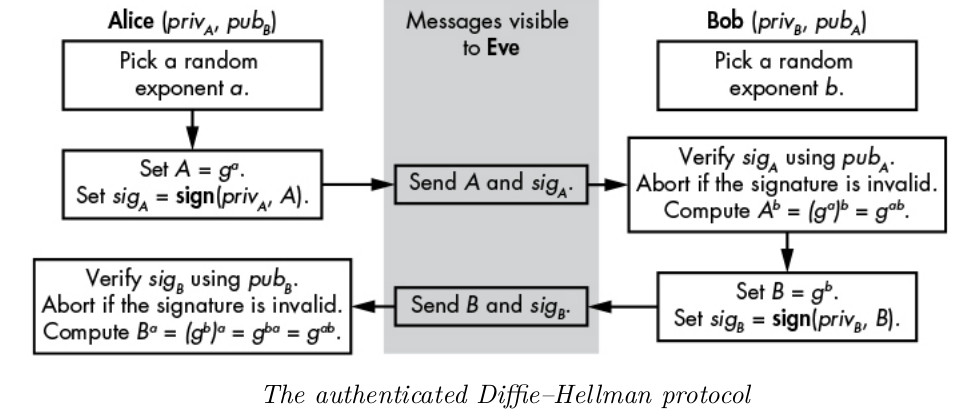
\includegraphics[width=0.8\textwidth]{authDH.jpg}
\end{center}
In generale in un protocollo per lo scambio sicuro di chiavi, c'è la necessità che almeno una delle due parti disponga di un \textbf{long-term secret} come può essere uno chiave \textbf{RSA}, ma a questo punto perché non usare direttamente una crittografia asimmetrica invece che un protocollo di scambio chiavi. Questo tipo di approccio \textbf{non} garantisce \textbf{\textit{forward-secrecy}}. \\
La \textbf{\textit{Forward Secrecy}} è una proprietà dei protocolli di \textit{negoziazione delle chiavi} che assicura che se una chiave di cifratura a lungo termine (\textit{long-term secret}) viene compromessa, le chiavi di sessione generate a partire da essa rimangono riservate. \\ \newline
\textbf{\textit{Ephemeral Diffie-Hellman Keys}} \\
In \textbf{\textit{TLS 1.3}} le chiavi simmetriche sono invece generatea partire da \textit{chiavi DH effimere}, questo implica che la chiave pubblica e privata dopo essere usate una sola volta, vengono \textbf{scartate da client e server}.

\newpage

\section{ElGamal}
Nel 1985 \textbf{\textit{ElGamal}} propone un sistema crittografico a chiave pubblica, questo viene pubblicato qualche anno dopo \textbf{RSA} (1977), ma lo affronteremo prima per una similitudine con \textit{Diffie-Hellman}. Poiché non venne brevettato, il sistema crittografico di \textit{ElGamal} venne inserito, insieme al protocollo \textbf{DSA} (\textit{Digital Signature Algorithm}), in molte suite crittografiche, tra tutte: \textbf{\textit{GNUPG}}. All'interno di \textit{ElGamal} possiamo identificare, come in qualunque altro algoritmo di crittografia asimmetrica due elementi:
\begin{enumerate}
    \item \textbf{generazione di una coppia di chiavi}, pubblica (che può essere resa disponibile) e privata.
    \item processo di comunicazione, composto a sua volta dalla \textbf{cifratura} e \textbf{decifratura}.
\end{enumerate}
\   \\
Per la parte di generazione della coppia di chiavi, inizialmente, \textit{Alice} determina i \textit{parametri} del protocollo:
\begin{itemize}
    \item un \textit{numero \textbf{p} primo} di lunghezza appropriata.
    \item una \textit{radice primitiva \textbf{g}} di $\mathbb{Z}_p^*$.
    \item calcolare il valore $A = g^a \bmod p$ dove $a \in \mathbb{Z}_p^*$ è un numero scelto uniformemente a caso.
\end{itemize}
Una volta determinati i paramentri \textit{Alice} conserverà \textit{a} come \textbf{chiave segreta} e provvederà a diffondere la terna \textit{(p, g, A)} come corrispondente \textbf{chiave pubblica}. Come possiamo notare, per questa prima parte del protocollo la differenza con \textit{DH} è solo nei destinatari della comunicazione, infatti non è più solo \textit{Bob} ma tutti. Nel momento in cui \textit{Bob} vuole inviare un messaggio cifrato ad \textit{Alice}, \textit{Bob} ottiene la chiave pubblica di \textit{Alice}, ovvero la terna \textit{(p, g, A)} e, dopo aver scelto un valore $b \in \mathbb{Z}_p^*$ uniformemente a caso, si calcola due quantità:
\begin{enumerate}
    \item $B = g^b \bmod p$
    \item $Cipher = (A^b * M) \bmod p$ dove M è il messaggio che \textit{Bob} vuole inviare ad \textit{Alice}.
\end{enumerate}
Inviando ad \textit{Alice} la coppia $C = (B, c)$ che costituisce il messaggio cifrato. Una volta ottenuto la coppia $(B, c)$ che costituisce il messaggio cifrato \textit{Alice} potrà decifrare il messaggio calcolando per prima cosa $Z = B^a \bmod p$ riuscendo ad ottenere attraverso l'uso del \textit{teorema di Euclide Esteso} il valore $Z^{-1} \bmod p$ e riuscendo a riottenere il messaggio in chiaro $M = (Z^{-1} * c) \bmod p$, si noti che il messaggio deve essere interpretabile come un numero \textbf{minore di p}. La \textbf{correttezza} dell'algoritmo è conseguenza del fatto che $Z = B^a \bmod p = A^b \bmod p$, ed è esattamente la stessa dimostrazione avvenuta per il teorema di \textit{diffie-hellman}.
\\ \newline
L'\textbf{Efficenza} è dovuta che la complessità della cifratura è dominata da due calcoli di potenze modulari, a cui va aggiunto il prodotto, mentre per il resto si tratta di pre-computazione delle chiavi. Al contrario la decifratura richiede il calcolo di una potenza, di un inverso e di una moltiplicazione. Un numero sostanzialmente molto ridotto di operazioni onerose che però bisogna considerare su numeri di oltre 1000 bit. Nel caso in cui il messaggio fosse più lungo della lunghezza del modulo \textit{p}, \textit{Bob} dovrebbe spezzare il messaggio in blocchi e ripetere la cifratura usando un valore di \textit{k} diverso per ogni singolo blocco. Con molti blocchi, e quindi con messaggi molto lunghi, cifratura e decifratura asimmetrica diventano dei passaggi molto onerosi soprattuto se confrontati con processi di cifratura simmetrica che oggigiorno supportano anche accelleratori hardware. Per questa ragione, la crittografia asimmetrica viene utilizzata in sinergia a quella simmetrica, in particolare, protocolli \textit{asimmetrici} vengono utilizzati in fase di \textit{autenticazione} delle parti e per lo \textit{scambio di chiavi}, mentre per la \textit{comunicazione} vera e propria viene utilizzato un protocollo \textit{simmetrico}. \\
Andando ad osservare invece la \textbf{Sicurezza} di \textit{ElGamal}, questa si basa sulla \textit{Computational Diffie-Hellman Assumptions} (\textbf{CDHA}) ovvero girando il problema che supponendo di riuscire a rompere \textit{ElGamal} e quindi di essere in grado di risolvere l'assunzione \textbf{\textit{CDH}}, infatti \textit{ElGamal} ``oscura'' il messaggio moltiplicando ($\times_p$) proprio per una quantità $A^b \bmod p$ che corrisponde al \textbf{segreto condiviso di DH}. Se dunque siamo in grado di decifrare \textit{M} (senza utilizzare il calcolo diretto del logaritmo discreto $a = \log_{g}{M} \bmod p$) allora possiamo risalire alla quantità $A^b \bmod p = g^{ab} \bmod p$ ovvero proprio la quantità che la \textbf{\textit{CDH Assumptions}} chiede di calcolare. Se quindi vale l'ipotesi \textit{CDHA} possiamo dedurre che \textbf{ElGamal è SICURO}. \\
Un errore da non commettere è di utilizzare per cifrature differenti lo stesso valore \textit{b}, infatti se questo dovesse valere, allora anche \textit{B} non cambia, quindi le cifrature di $M_1 \text{ e } M_2$ risulterebbero:
\begin{center}
    $C_1 = (B, c_1 = (A^b * M_1) \bmod p) \qquad \text{ e } \qquad C_2 = (B, c_2 = (A^b * M_2) \bmod p)$ \\
    Consideriamo ora $C_1$ \\\   \newline
    \begin{math}
        \begin{aligned}
            C_1 &= (B, c_2) \\
            &= (g^b \bmod p,\;A^b * M_1 \bmod p) \\
            &= (g^b \bmod p,\;g^{ab} * M_1 \bmod p) \\
            &= (g^b \bmod p,\;Z * M_1 \bmod p) \qquad Z = B^a \bmod p = g^{ab} \bmod p
        \end{aligned}
    \end{math}    
\end{center}
\begin{center}
    $c_2 = Z * M_2 \bmod p \qquad M_2 = Z^{-1} * M_2 \bmod p$ \\
    Moltiplichiamo a destra e a sinistra per $c_1^{-1}$ \\
    \begin{math}
        \begin{aligned}
            c_1^{-1} * c_2 \bmod p &= c_1^{-1} * (Z * M_2) \bmod p \\ 
            &= (A^b * M_1)^{-1} * (Z * M_2) \bmod p \\
            &= (g^{ab} * M_1)^{-1} * (Z * M_2) \bmod p \\
            &= (Z * M_1)^{-1} * (Z * M_2) \bmod p \\
            &= Z^{-1} * Z * (M_1^{-1} * M_2) \bmod p \\
            &= (M_1^{-1} * M_2) \bmod p \\
        \end{aligned}
    \end{math}
\end{center}
\begin{center}
    Moltiplichiamo a destra e a sinistra per $M_1$ \\
    \colorbox{yellow}{$M_2 = M_1 * (c_1^{-1} * c_2) \bmod p$}
\end{center}
Se \textit{Eve} fosse in grado (per qualsiasi motivo) di decifrare il messaggio $M_1$, e quindi avere la coppia $(M_1, \; c_1)$ potrebbe decifrare anche i successivi messaggi cifrati con lo stesso valore \textit{b}.

\newpage
\section{Sistema Crittografico RSA}
Il sistema crittografico \textbf{RSA} prende il nome dalle iniziali dei loro inventori: \textit{Ronald L. Rivest}, \textit{Adi Shamir} e \textit{Leonard M. Adlemam}. \textit{RSA} basa la sua efficacia, in termine di \textbf{sicurezza}, sulla difficoltà computazionale del \textbf{problema della fattorizzazione di numeri interi}, ovvero sul fatto che ad oggi non esistono algoritmi efficienti per fattorizzare numeri di grandi dimensioni. Ad oggi, però, non esiste un argomentazione matematica, come nel caso di \textit{Diffie-Hellman}, che dimostri che saper violare efficientemente RSA implichi saper fattorizzare numeri interi. \\
\textcolor{violet}{\textbf{\textit{Warning}}}: un \textbf{computer quantistico} sarebbe in grado di fattorizzare in maniera efficacie i numeri interi e quindi violare RSA.
\\ \newline
L'\textbf{Algoritmo in Dettaglio}: come in ogni cifrario asimmetrico la generazione delle chiavi è eseguita dal destinatario del ciphertext, che identificheremo come \textit{Alice}, il protocollo ha un solo parametro di input, che è la lunghezza in bit, indicata con \textit{N}, dell'intero con cui si effettuano le riduzioni modulari.
\begin{itemize}
    \item \textbf{Generazione delle Chiavi: \textit{Alice}}
    \begin{enumerate}
        \item generare due primi a casa \textit{p} e \textit{q} di lunghezza $\frac{N}{2}$.
        \item calcolare il prodotto $n = p * q$.
        \item calcolare $\phi(n) = (p - 1) * (q - 1)$.
        \item determinare un intero \textit{e}, (normalmente $e = 65537$) e relativamente primo con $\phi(n)$ ovvero che $gcd(e, \phi(n)) = 1$.
        \item calcolare l'inverso moltiplicativo \textit{d} di \textit{e} modulo $\phi(n)$, che esiste perché \textit{e} è \textbf{coprimo} con $\phi(n)$.
        \item diffondere la coppia (\textbf{\textit{e}}, \textbf{\textit{n}}) come \textbf{chiave pubblica} e conservare \textbf{\textit{b}} come \textbf{chiave privata}.
    \end{enumerate}
    \item \textbf{Cifratura del Messaggio M: \textit{Bob}}
    \begin{enumerate}
        \item si procura la chiave pubblica di \textit{Alice}, (\textbf{\textit{e}}, \textbf{\textit{n}}).
        \item calcola $C = M^e \bmod n$.
        \item invia \textit{C} come messaggio cifrato ad \textit{Alice}.
    \end{enumerate}
    \item \textbf{Decifrazione del Messaggio C: \textit{Alice}} calcola $M = C^d \bmod n$.
\end{itemize}
\   \\
\textbf{Correttezza del Protocollo RSA} \\
Dobbiamo dimostrare che $M = C^d \bmod n$, avremo bisogno durante la procedura dell'ugualianza: 
\begin{center}
    $e \cdot d = k \cdot \phi(n) + 1$ \\
    $d = e^{-1} \bmod \phi(n)$ \\
    $e \cdot d = e \cdot e^{-1} \bmod \phi(n)$ \\
    $e \cdot d = 1 \bmod \phi(n)$ \\
    $e \cdot d = k \cdot \phi(n) + 1$ \\
\end{center}
Infatti ricordiamo che \textit{d} è l'inverso moltiplicativo di \textit{e} modulo $\phi(n)$ e questo vuol dire che il prodotto $e \cdot d - 1$ è un multiplo di $\phi(n)$ quindi possiamo scriverlo come $k \cdot \phi(n)$.
\begin{center}
    \begin{math}
        \begin{aligned}
            C^d \bmod n &= (M^e \bmod n)^d \bmod n \\
            &= M^{e \cdot d} \bmod n \\
            &= M^{k \cdot \phi(n) + 1} \bmod n \\
            &= M \cdot M^{k \cdot \phi(n)} \bmod n \\
            &= M \cdot M^{k \cdot (p - 1) \cdot (q - 1)} \bmod n \\
            &= (M \cdot (M^{(p-1)})^{k \cdot (q - 1)}) \bmod n 
        \end{aligned}
    \end{math}
\end{center}
Possiamo verificare l'ugualianza:
\begin{center}
    $M \cdot M^{k \cdot (p - 1)(q - 1)} \bmod p = M \bmod p$
\end{center}
Infatti, se $M \bmod p = 0$ allora entrambi i membri sono uguali a \textit{0}, nel caso contrario, ovvero nel caso in cui $M \bmod p \neq 0$ che:
\begin{center}
    \begin{math}
        \begin{aligned}
            (M \cdot M^{k \cdot (p - 1)(q - 1)}) \bmod p &= (M \cdot (M^{(p - 1)^{k \cdot (q - 1)}})) \bmod p \\
            &= (M \cdot (M^{p - 1} \bmod p)^{k \cdot (q - 1)}) \bmod p \\
            &= (M \cdot (1)^{k \cdot (q - 1)}) \bmod p\;||\;\Leftarrow \text{per il piccolo teorema di Fermat} \\
            &= M \bmod p
        \end{aligned}
    \end{math}
\end{center}
Allo stesso modo vale in maniera \textit{equivalente}:
\begin{center}
    $M \cdot M^{k \cdot (p - 1)(q - 1)} \bmod q = M \bmod q$
\end{center}
Le quantità $C^d$ e \textit{M} sono congrue sia in $\bmod p$ che in $\bmod q$, in altri termini le quantità $C^d$ e \textit{M} hanno gli stessi \textbf{resti} nella divisione con \textit{p} e \textit{q}, ma poiché $gcd(p, q) = 1 \land p \cdot q = n$ e utilizzando il \textbf{\textit{Chinese remainder theorem}} avremo che \colorbox{yellow}{$C^d \equiv M \bmod n$} riuscendo a verificare la \textbf{reversibilità} di RSA.
\\ \newline
\textbf{Efficenza}
\newline
A differenza di \textit{DH} e quindi non necessitando che \textit{p} e \textit{q} siano generati come \textit{strong prime}, ovvero $p,q = 2*k + 1$ fa in modo che \textit{p} e \textit{q} possano essere determinati velocemente. Andando ad analizzare la creazione della della \textit{chiave pubblica} e della \textit{chiave privata}, queste computazioni vengono eseguite una sola volta. Cifratura e decifratura richiedono calcoli esponenziali modulari, che sono operazioni \textit{efficentemente implementate} ma che coinvolgono numeri non gestibili in aritmentica di macchina. Ci interessa trovare un \textit{e} adatto ai nostri scopi, ovvero che siamo \textbf{coprimo} con $\phi(n)$.
\begin{itemize}
    \item scegliere un numero $e > max\{p, q\}$, infatti andando a calcolare $\phi(n) = (p - 1) \cdot (q - 1)$ avremo che i fattori di $\phi(n)$ sono tutti minori di \textit{p} e \textit{q}. 
    \item procedere per ``tentativi casuali'', grazie al fatto che il calcolo del \textit{MCD} è molto rapido.
    \item fissare a priori un esponente piccolo  (\textit{3} o \textit{5}) e continuare a generare primi \textit{p} e \textit{q} fino a quando non si verifica la condizione $gcd(e, (p - 1) \cdot (q - 1)) = 1$, nelle implementazioni \textbf{reali} si procede in questo modo partendo da un \textit{e} più elevato.
\end{itemize}
\   \\
La \textbf{Sicurezza} di RSA risiede, dal punto di vista strettamente \textit{matematico}, della difficoltà di \textbf{fattorizzare} numeri interi di grandi dimensioni, infatti se ne esistessero \textit{Eve} potrebbe ottenere \textit{p} e \textit{q} in modo da otterene prima $\phi(n)$ e successivamente \textit{d}. Il viceversa non è dimostrato, non si è stati però in grado di violare efficaciemente RSA attraverso la fattorizzazione di \textbf{\textit{n}}. Altra faccenda è invece parlare della \textbf{correttezza implementativa} di RSA. \\
Andiamo ora ad elencare alcune \textbf{vulnerabilità} nel caso in cui RSA sia impletato in maniera errata:
\begin{itemize}
    
    \item \textbf{Malleabilità}: ricordiamo che un algoritmo di cifratura \textbf{\textit{E}} è \textit{malleabile} se dato un testo cifrato $C_1 = E(M_1)$ è possibile creare un secondo testo cifrato $C_2 = E(M_2)$ tale per cui ci sia una \textit{corrispondenza ``significativa''} tra $M_1$ e $M_2$. Il protocollo RSA di base è \textbf{malleabile}. In questo caso avremo un attacco del tipo \textbf{\textit{Chosen Ciphertext Attack}} infatti il prodotto di due ciphertext corrisponde al prodotto di due plaintext. Per dimostrarlo andiamo a definire un testo cifrato $C_1 = M_1^e \bmod n$, a questo punto creiamo un testo cifrato ``intermedio'', ad esempio con $M_1' = 2$ avremo che $C_1' = 2^e \bmod n$. Possiamo quindi ottenere $C_2 = C_1 * C_1' = (M_1^e \bmod n) \cdot (M_1'^e \bmod n) = (M_1 \cdot M_1')^e \bmod n$ ovvero un ciphertext arbitrario, nel caso sia present un \textit{Decipher Oracle} potremmo decifrare il nostro $C_2$ a quel punto abbiamo facilmente modo di ottenere $M_1$:
    \begin{center}
        \begin{math}
            \begin{aligned}
            C_2^d \bmod n &= (C_1 \cdot C_1')^d \bmod n \\
            &= ((M_1^e \bmod n) \cdot (2^e \bmod n))^d \bmod n \\
            &= ((M_1^e)^d \cdot (2^e)^d) \bmod n \\
            &= (M_1 \cdot 2) \bmod n
            \end{aligned}    
        \end{math}    
    \end{center}
    È quindi possibile moltiplicare per l'inverso $M_1' \bmod n$ per ottenere l'$M_1$ desiderato. In letteratura questo tipo di attacco è anche nota come proprietà \textbf{\textit{Omomorfica}}.

    \item \textbf{Caso di \textit{e} troppo piccolo}: nel momento in cui \textit{e} è troppo piccolo e contemporaneamente il testo da cifrare è anch'esso molto breve, in quest'ottica se \textit{e = 3} e il messaggio è breve può succedere che $M^e < n$, in questo caso succede che il modulo \textit{n} non riduca il risulta di $M^e \bmod n$ e che quindi avremo che $C = M^e$. In questo caso \textit{Eve} può calcolare la radice cubica di \textit{C}. Per questa ragione, lo standard \textbf{\textit{FIPS}} prevede che \textit{e} non sia minore di $2^{16} + 1 = 65537$. Questa problematica unita a quella precedente possono portare a tipologie di attacco del tipo: \textbf{\textit{Hastad's Broadcast Attack}} (bisogna combinare le due vulnerabilità tramite il \textit{CRT}).

    \item \textbf{Possibilità di Fattorizzare \textit{n}}: nel caso in cui \textit{p} e \textit{q} vengano scelti con caratteristiche non idonee è possibile modellarli in modo tale da ottenere la fattorizzazione di \textit{n}. Identifichiamo come \textbf{malconfigurazione} il fatto che \textit{p} e \textit{q} vengano scelti \textbf{``molto vicini''}. Andiamo ad analizzare il contesto:
    \\
    $n = p * q \;\;\; \Rightarrow p \neq q$ possiamo dire che: $p > q$ \\
    \begin{center}
        \begin{math}
            \begin{aligned}
                n &= (\frac{p + q}{2})^2 - (\frac{p - q}{2})^2 \\
                &= \frac{p^2 + q^2 + 2pq - p^2 -q^2 + 2pq}{4} \\
                &= \frac{4 * pq}{4} = p \cdot q
            \end{aligned}
        \end{math}
    \end{center}
    È quindi possibili visualizzare \textit{n} come differenza di quadrati del tipo $n = x^2 -y^2$, per poter utilizzare questa nozione per portare un attacco su RSA dobbiamo cercare di capire con quanta facilità è possibile calcolare la quantità: $\frac{p + q}{2}$ o $\frac{p - q}{2}$ senza ovviamente conoscere \textit{p} e \textit{q}. La possibilità più immediata è quella di tentare un \textit{brute-force} che permettere iterando su una delle due (ad esempio $x^2$) di ottenere l'altra. Calando ad ogni iterazione $y^2 = x^2 -n$. Andando nel dettaglio:
    \begin{enumerate}
        \item assegnamo a $x_0$ un valore arbitrario $x'$. Il valore iniziale di \textit{x} deve essere sensato per il caso d'uso, consideriamo quindi:
        \begin{center}
            $\frac{p + q}{2} > \sqrt{n}$ \\
            $\Rightarrow \; x' = \ceil{\sqrt{n}}$
        \end{center}
        \item calcoliamo la quantità $z_i = x_i^2 - n$. Nel caso in cui $z_i$ è un quadrato perfetto in $\mathbb{Z}_n$ allora passiamo al punto \textit{4}.
        \item Poniamo $x_i = x_{i - 1} + 1$ e torniamo al passo precedente.
        \item possiamo calcolare e restituire i due fattori: $x + \ceil{\sqrt{z_i}}$ e $x - \ceil{\sqrt{z_i}}$.
    \end{enumerate}
    Analizzando questo attacco a \textit{forza bruta} è interessante andare a calcolare sotto quali condizioni l'algoritmo riesca a \textbf{fattorizzare} in ``tempi ragionevoli''. Ovvero che la differenza tra \textit{p} e \textit{q} risulti $\mathcal{O}(\sqrt[4]{n})$, in termini di cifre significa che \textit{p} e \textit{q} coincidano nelle metà più significative.

    \item \textbf{Vulnerabilità Dipendenti dai Generatori Casuali}: nel 2012 è stato fatto uno studio su 4.7 milioni di moduli RSA di 1024 bit ed è risultato che i dublicati non sono infrequenti e in alcuni casi (12720) si è notato che i due moduli avevano un fattore in comune, questo permetterebbe la fattorizzazione di ben due \textit{n} e quindi l'inutilià della chiave pubblica generata in quanto chiunque riuscirebbe a leggere il ciphertext. Infatti è sufficiente calcolare $gcd(n_1, n_2) = f$, dove \textit{f} è il fattore primo in comune per riuscire ad ottenere prima $\phi(n)$ e successivamente \textit{d}. La causa di questo attacco è da imputare per la maggiore alle \textbf{debolezze dei generatori (pseudo)casuali} coinvolti nella scelta dei numeri primi

\end{itemize}
\   \\
È quindi importante, per non incorrere in vulnerabilità di applicare \textbf{aspetti implementativi} apparentemente marginali, ma che bisogna tenere in considerazione quando si va a sviluppare un architettura che si basa su \textbf{RSA}. Quali:
\begin{itemize}
    \item la \textbf{generazione} di \textbf{numeri casuali} deve essere effettuata dopo che si ha accumulato abbastanza \textbf{entropia} da garantire che le eventuali collisioni non abbiano probabilità maggiore di quanto previsto teoricamente.
    \item i fattori \textit{p} e \textit{q} non devono essere troppo vicini per evitare che venghino fattorizzati tramite l'\textbf{algoritmo di fattorizzazione di Fermat}.
    \item gli esponenti \textit{e} e \textit{d} non devono essere piccoli, per evitare di rendere inefficace la riduzione in modulo \textit{n}.
    \item la malleabilità del protocollo deve essere eliminata con opportuni accorgimenti.
\end{itemize}
\   \\
\textbf{Miglioramente dell'efficienza di RSA} \\
È possibile effettuare in due modi diversi un'ottimizzazione.
\begin{enumerate}
    \item il primo lavora nel momento della \textbf{cifrazione} ovvero durante il calcolo $C = M^e \bmod n$, infatti sappiamo che l'esponenziale modulare non è altro che uno shift di \textit{m} posizioni in base alle posizioni dei bit \textit{non 0}, secondo il \textbf{FIPS} viene raccomandato che \textit{e} non sia minore di \textbf{65537}, in molti casi reali la scelta ricade proprio su questo numero in quanto può essere rappresentato come $(2^{16} + 1)_{(10)} = 10000000000000001_{(2)}$ e proprio la presenza di molte cifre a $0$ rende \textbf{più efficiente il calcolo dell'esponenziale modulare}.

    \item il secondo metodo riguarda invece la fase di \textbf{decifrazione} infatti è previsto che \textit{Alice} ricavi il plaintext tramite $M = C^d \bmod n$ possiamo però utilizzare il \textbf{\textit{CRT}} per ridurre la dimensione degli esponenti.
    \begin{center}
        $M_p = C^d \bmod p \;\;\; \text{e} \;\;\; M_q = C^d \bmod q$ \\
        e possiamo risalire al valore di \textit{M} tramite: \\
        $M = ((q \cdot (q^{-1} \bmod p)) \cdot M_p + (p \cdot (p^{-1} \bmod q)) \cdot M_q) \bmod n$ \\
        in cui i coefficenti $q \cdot (q^{-1} \bmod p)$ e $p \cdot (p^{-1} \bmod q)$ possono essere precalcolati.
    \end{center}
    È possibile ottimizzare in maniera maggiore precalcolando $s = d \bmod {(p - 1)}$ e $t = d \bmod {(q - 1)}$. Possiamo analizzare che $d = s + a \cdot (p - 1)$ e che dunque possiamo semplificare i calcoli:
    \begin{center}
        \begin{math}
            \begin{aligned}
                C^d \bmod p &= C^{s + a \cdot (p - 1)} \bmod p \\
                &= C^s \cdot {C^{(p - 1)}}^a \bmod p \\
                &= C^s \cdot 1^a \bmod p \\
                &= C^s \bmod p = M_p
            \end{aligned}
        \end{math}
    \end{center}
    Possiamo svolgere gli stessi calcoli, analogamente, per \textit{t} andando a sostituire il modulo \textit{p} con il valore \textbf{\textit{q}} andando ad ottenere: $M_q = C^t \bmod q$. E quindi calcolando $M_p$ ed $M_q$:
    \begin{center}
        $M_p = C^s \bmod p \;\;\; \text{e} \;\;\; M_q = C^t \bmod q$
    \end{center}
    Questa computazione permette di calcolare gli esponenziali su numeri di grandezza dimezzata.
\end{enumerate}
\   \\
\textbf{\textit{Optimal Asymmetric Encryption Padding - OAEP}} \\
Permette di aggiungere alla cifratura di RSA un informazione addizionale chiamata \textbf{padding}, costituita da sequenze \textit{(pseudo)casuali} ed è quindi sempre più determinante avere dei generatori affidabili. \\ 
\begin{center}
    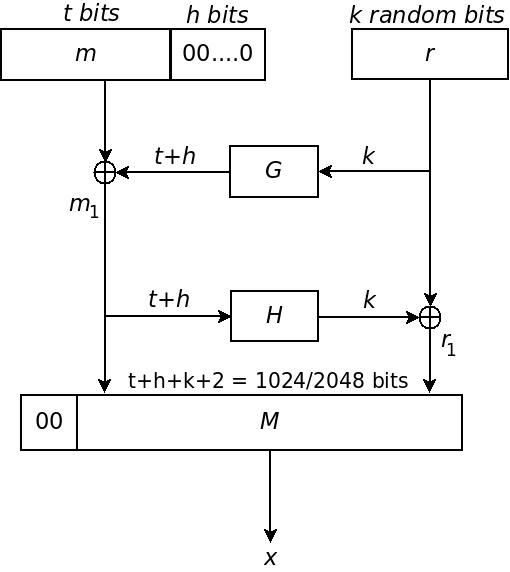
\includegraphics[width=0.45\textwidth]{OAEP.jpg}
\end{center}
Consideriamo \textit{n} è il numero di bit nel modulo RSA, \textit{h} e \textit{k} sono costanti intere fissate dal protocollo ed \textit{m} è il messaggio in chiaro, ovvero una stringa lunga $n - k - h - 2$. Definiamo ora \textbf{\textit{G}} e \textbf{\textit{H}} come due funzioni di \textit{hash crittografico}. Andiamo ad analizzare i passaggi per cifrare:
\begin{enumerate}
    \item al messaggio \textit{m} va applicato un \textit{padding} di \textit{h} zeri per arrivare alla lunghezza di $n - k - 2$
    \item definiamo \textit{r} come una stringa casualmente generata di \textit{k} bit
    \item \textit{r} verrà poi espansa da \textit{k} a $n - k - 2$ bit tramite la funzione di hash \textbf{\textit{G}}
    \item $m_1 = m \oplus G(r)$
    \item tramite \textbf{\textit{H}} $m_1$ viene ridotta da $n - k - 2$ bit a \textit{k} bit.
    \item $r_1 = r \oplus H(m_1)$
    \item il messaggio finale, che verrà successivamente convertito in un numero \textit{x} da mandare come input ad RSA è ``$00\;||\;m_1\;||\;r_1$''
\end{enumerate}
La \textbf{decifrazione} è definita dalle proprietà dello \textbf{\textit{xor}} logico.

\newpage
\section{Sistema Crittografico Asimmetrico di Rabin}
Poco dopo l'introduzione di \textit{RSA}, \textbf{Michael O. Rabin} ha sviluppato un algoritmo crittografico a cui appartiene la proprietà teorica di essere equivalente alla fattorizzazione, ovvero un algoritmo \textit{polynomial time} in grado di violare il sistema di \textit{Rabin} potrebbe essere utilizzato per la fattorizzazione di interi (e viceversa), ma, come contro, presenta una limitazione in quanto la decifrazione di un ciphertext arbitrario produce \textbf{quattro possibili} candidati come \textbf{plaintext}. Andiamo ad analizzare le quattro possibili radici di un numero $y \in \mathbb{Z}_p^*$ attraverso un esempio numerico.
\begin{center}
    Definiamo: $p = 13 \;\; q = 23 \;\; n = p \cdot q = 299$ \\
    Prendiamo un elemento $x \in \mathbb{Z}_p^*$: $x = 27$ \\
    Calcoliamo il suo quadrato: $ y = x^2 \bmod n = 131$ \\  
    Sappiamo che in $\mathbb{R} \Rightarrow \sqrt{131} = \pm x$ \\
    Allora anche in $\mathbb{Z}_n^*$ saranno presenti due radici: $(x, -x)$ \\
    Calcoliamo $-x = n - x = 272 \Rightarrow (-x)^2 \bmod n = 131$ \\
    Precalcoliamo $c_p = q \cdot (q^{-1} \bmod p) = 92 \;\;\; c_q = p \cdot (p^{-1} \bmod q) = 208$
\end{center}
Consideriamo ora che $n = p \cdot q$ utilizzando il \textit{CRT} sappiamo che data l'equazione $\exists \: C \; | \; C \equiv y \bmod n, \; C = c_p * a_1 + c_q * a_2$, prima di tutto andiamo a calcolarci le quantità $a_1 \text{ e } a_2$, come $a_i = y \bmod n_i, \;\; i = \{p, q\}$, $a_1$ è il corrispondente di \textit{y} in $\mathbb{Z}_p^*$ e, ovviamente $a_2$ è il corrispondente di \textit{y} in $\mathbb{Z}_q^*$. Allora sia per $a_1 \text{ che per } a_2$ saranno presenti 2 radici, rispettivamente in $\mathbb{Z}_p^*$ e in $\mathbb{Z}_q^*$, possiamo calcolarli come:
\begin{center}
    $x_{p^1} = y^{(2^{-1} \bmod p)} \bmod p = 1$ \\
    $-x_{p^1} = x_{p^2} = p - x_{p^1} = 12$ \\
    $x_{q^1} = y^{(2^{-1} \bmod q)} \bmod q = 4$ \\
    $-x_{q^1} = x_{q^2} = q - x_{q^1} = 19$ \\
    Per trovare le radici di \textit{y} in $\mathbb{Z}_n^*$ applicando il \textbf{\textit{CRT}} avremo: \\
    $x_1 = c_p * x_{p^1} + c_q * x_{q^1} = 27$ \\
    $x_2 = c_p * x_{p^1} + c_q * x_{q^2} = 157$ \\
    $x_3 = c_p * x_{p^2} + c_q * x_{q^1} = 142$ \\
    $x_4 = c_p * x_{p^2} + c_q * x_{q^2} = 272$ \\
\end{center}
Alla fine avremo che $y = x_i^2 \bmod n = 131\;\; \forall i = 1, 2, 3, 4$, siamo riusciti a ``dimostrare'' che preso un \textit{quadrato perfetto} in $\mathbb{Z}_n*$ con \textit{n} che è il prodotto di due numeri \textit{coprimi} tra loro, il quadrato perfetto avrà quattro \textbf{radici} in $\mathbb{Z}_n*$, due delle quali saranno fra loro \textbf{congrue modulo p} e due \textbf{congure modulo q}. Riuscendole ad ottenere applicando il \textit{CRT}.
\\ \newline
Descriviamo ora l'\textbf{algorimo generale}, anche in questo caso verrà diviso in generazione delle chiavi, che necessita come input un solo parametro, ovvero la lunghezza in bit di \textit{n}. E una parte di scambio di informazioni che quindi necessiterà di utilizzare cifratura e decifratura.
\begin{itemize}
    \item \textbf{Generazione delle chiavi: \textit{Alice}}
    \begin{enumerate}
        \item genera due numeri primi a caso di lunghezza $\frac{n}{2}$ bit tale che $p \equiv 3 \bmod 4$ e $q \equiv 3 \bmod 4$.
        \item calcolo di $n = p \cdot q$.
        \item diffonde \textit{n} come \textbf{chiave pubblica} e conserva la coppia \textit{(p, q)} come \textbf{chiave segreta}.
    \end{enumerate}
    \item \textbf{Cifratura di un messaggio: \textit{Bob}}
    \begin{enumerate}
        \item si procura la chiave pubblica \textit{n} di \textit{Alice}.
        \item calcola $C = M^2 \bmod n$.
        \item invia \textit{C} ad \textit{Alice} come messaggio cifrato.
    \end{enumerate}
    \item \textbf{Decifrazione del messaggio \textit{C}: \textit{Alice}}
    \begin{enumerate}
        \item \textit{Alice} calcola $M_p = C^{\frac{p + 1}{4}} \bmod p$ e $M_q = C^{\frac{q + 1}{4}} \bmod q$, notiamo che $M_p$ è una delle \textit{radici quadrate di C} modulo \textit{p} perché:
        \begin{center}
            \begin{math}
                \begin{aligned}
                    M_p^2 \bmod p &= (C^{\frac{p + 1}{4}})^2 \bmod p \\
                    &= C^{\frac{p + 1}{2}} \bmod p \\
                    &= C^{\frac{p - 1}{2}} \cdot C \bmod p \\
                    &= ((M^2 \bmod n)^{\frac{p - 1}{2}} \cdot C) \bmod p \\
                    &= (((M^2 \bmod n) \bmod p)^{\frac{p - 1}{2}} \cdot C) \bmod p \\
                    &= ((M^2 \bmod p)^{\frac{p - 1}{2}} \cdot C) \bmod p \\
                    &= (M^{p - 1} \cdot C) \bmod p \\
                    &= (1 \cdot C) \bmod p \\
                    &= C \bmod p
                \end{aligned}
            \end{math}
        \end{center}
        Analogamente $M_p$ è una delle \textit{radici quadrate di C} modulo \textit{q}.
        \item riprendendo il discorso del \textit{CRT} possiamo calcolare le quattro radici di $C$ modulo \textit{n} e una di questi valori sarà il messaggio originale.
        \begin{center}
            $M_1 = ((q \cdot (q^{-1} \bmod p)) * M_p) + (p \cdot (p^{-1} \bmod q) * M_q) \bmod n = (c_p \cdot M_p + c_q \cdot M_q) \bmod n$ \\
            $M_2 = n - M_1 = ((-c_p) \cdot M_p + (-c_q) \cdot M_q) \bmod n$ \\
            $M_3 = ((q \cdot (q^{-1} \bmod p)) * M_p) - (p \cdot (p^{-1} \bmod q) * M_q) \bmod n = (c_p \cdot M_p + (-c_q) \cdot M_q)$ \\
            $M_4 = n - M_3 = ((-c_p) \cdot M_p + c_q \cdot M_q) \bmod n$ 
        \end{center}
        Utilizzando il \textit{CRT} possiamo verificare che, effettivamente, \textit{M} è effettivamente una delle quattro radici di \textit{C} modulo \textit{n}.
    \end{enumerate}
\end{itemize}
\   \\
\textbf{Equivalenza con il problema della fattorizzazione}
\newline
Dobbiamo dimostrare che se siamo in grado di decifrare (con un incertezza 1 su 4) allora possiamo fattorizzare \textit{n}, il viceversa è ovvio. Abbiamo visto che le quattro radici di $C \bmod n$ corrispondono alle quattro possibili combinazioni delle due radici modulo \textit{p} e delle due radici modulo \textit{q}:
\begin{enumerate}
    \item $M_1$ corrisponde alla coppia $(M_p, M_q) = (C^{\frac{p + 1}{4}} \bmod p, C^{\frac{q + 1}{4}} \bmod q)$.
    \item $M_2$ corrisponde alla coppia $(p - M_p, q - M_q)$ .
    \item $M_3$ corrisponde alla coppia $(M_p, q - M_q)$.
    \item $M_4$ corrisponde alla coppia $(p - M_p, M_q)$.
\end{enumerate}
L'obiettivo è fattorizzare un numero \textit{n} dato in input e considerare di possedere una scatola \textbf{black-box} che contenga l'algoritmo di dato un numero \textit{C}, resido quadratico in modulo \textit{n}, restituirti una delle quattro radici. \\
La riduzione è un algoritmo tipo \textbf{Las Vegas} e funziona in questo modo:
\begin{enumerate}
    \item genero a caso un numero $r \in \mathbb{Z}_n, r \neq 0$.
    \item se $m = gcd(r, n) \neq 1$ restituisco \textit{m} e \textit{n/m}.
    \item altrimenti considero \textit{r} come un ``messaggio'', calcolo $C = r^2 \bmod n$ e sottopongo \textit{C} alla black box.
    \item se $r'$ è il valore restituito dalla black-box, calcolo $m = gcd(r - r', n)$.
    \item se $m > 1 \text{ e } m \neq n$ restituisco i fattori \textit{m} e \textit{n/m}, altrimenti ritorno al passo \textit{1}.
\end{enumerate}
La correttezza è che la \textit{black-box} ritorna $r'$ che è una delle quattro radici di $C = r^2 \bmod n$ e che può essere uno dei quattro modi che abbiamo per combinare le due radici di $r^2 \bmod p$ e le due radici di $r^2 \bmod q$. Consideriamo che $r = (r_p, r_q) = (M_p, M_q)$ (esempio senza perdere di generalità).
\begin{enumerate}
    \item $r' = (r_p, r_q) = r$ allora avremo che $r - r' = 0$ ovvero che seguendo il \textit{CRT} avremo che $(r - r') \bmod p = r_p - (p - r_p) \bmod p = 2r_p \bmod p$ e che $(r -r') \bmod q = r_q - (q - r_q) \bmod q = 2r_q \bmod q$ e che quindi $n = m$ e che quindi non riusciamo a ad ottenere una risposta dall'algoritmo.
    \item $r' = (-r_p, -r_q) = -r$ allora avremo che $r - r' = 2r$ e quindi otteniamo $gcd(r, n) = 1$ e anche qui non riusciamo a determinare i fattori di \textit{n}.
    \item $r' = (r_p, - r_q)$ allora avremo che $r - r' = (r_p, r_q) - (r_p, - r_q) = (r_p - r_p, r_q - (- r_q)) = (0, 2r_q)$ ma avere il fatto in modulo p a \textit{0} implica che nel \textit{CRT} il suo fattore modulo p sia $r_p = C^{\frac{p + 1}{4}} \bmod p = 0$ che implica che $C^{\frac{p + 1}{4}}$ sia multiplo con \textit{p} e quindi avremo che $gcd(r', n) = p$.
    \item $r = (-r_p, r_q)$ in questo caso avremo l'esatto opposto del punto precedente, ovvero che $r - r' = (2r_p, 0)$ in questo caso avremo che quindi nel fattore $r_p = C^{\frac{q + 1}{4}} \bmod q = 0$ del \textit{CRT} avremo che $C^{\frac{q + 1}{4}}$ sia multiplo con \textit{q} e quindi avremo che $gcd(r', n) = q$.
\end{enumerate}
\   \\
\textbf{Riduzioni Polinomiali} \\
Per riuscire a dimostrare che un algoritmo è ``uguale'' ad un altro, in questo caso dobbiamo dimostrare che l'\textbf{algoritmo di fattorizzazione} è ``uguale'' all'\textbf{algoritmo per la risoluzione di Rabin}, bisogna dimostrare che l'uno e l'altro abbiano uguale \textbf{complessità}. Nel caso di dimostrare che saper risolvere \textbf{Rabin} equivale a saper \textbf{FATTORIZZARE} è immediato infatti se sappiamo fattorizzare un  numero \textit{n} allora otteniamo \textit{p} e \textit{q} e quindi abbiamo la chiave privata di \textit{Alice}. Per dimostrare, invece, che risolvere \textbf{Rabin} vuol dire risolvere il problema della \textbf{FATTORIZZAZIONE} abbiamo utilizzato il sistema della \textbf{black box}, ovviamente affinché questo funzioni la \textit{black box} deve ritornare una della quattro radici in maniera casuale.
\chapter{Firma Digitale}
La \textit{firma digitale} è il metodo di \textbf{autenticazione} basato su crittografia a chiave pubblica. In generale si tratta di una \textbf{``cifratura''} con la \textbf{chiave privata}. L'\textbf{autenticità del mittente} deriva dal fatto che solo con la corrispondente \textbf{chiave pubblica del mittente} si possa decifrare un messaggio ``cifrato'' \textit{M}.

\section{Firma Digitale con RSA}
L'osservazione fondamentale è il ruolo perfettamente \textbf{simmetrico} degli esponenti \textit{e} e \textit{d}, infatti essi sono l'uno l'inverso dell'altro in $\mathbb{Z}_n^*$. È quindi possibile \textbf{\textit{firmare}} un messaggio \textit{M} con la propria \textbf{chiave privata}, in questo caso \textbf{non} avremo \textbf{riservatezza} sul messaggio, infatti essendo che il messaggio \textit{M} si potrà decifrare con la chiave pubblica, quindi nota a chiunque, essa servirà unicamente per validare che quel messaggio è stato inviato dal proprietario della corrispondente chiave privata.
\begin{center}
    $F = M^d \bmod n \;\;\;\;\; M = F^e \bmod n$
\end{center}
Naturalmente anche se un \textit{destinatario} decifrasse il messaggio \textit{F} con la chiave pubblica del \textit{mittente} non potrebbe validare il messaggio è quindi necessario associare alla quantità \textit{F} il messaggio originale \textit{M} per poter poi effettuare il confronto tra i due, ecco quindi derivata la ``definizione'' di \textbf{\textit{digital signature}}: $DS = (M, F)$. \\
La garanzia è che senza una copia di \textit{d} è computazionalmente intrattabile \textbf{forgiare} una coppia $(\overline{M}, \overline{F})$ dove $\overline{F} = \overline{M}^d \bmod n$.
\\ \newline
\textbf{Protocollo di Base}
\begin{itemize}
    \item \textbf{Firma del Messaggio: \textit{Alice}}
    \begin{enumerate}
        \item calcolo $F = M^d \bmod n$.
        \item invio della coppia $(M, F)$.
    \end{enumerate}
    \item \textbf{Verifica della Firma: \textit{Bob}}
    \begin{enumerate}
        \item ottiene la chiave pubblica di \textit{Alice} $(n, e)$.
        \item calcola $M' = F^e \bmod n$.
        \item accetta se e solo se $M = M'$.
    \end{enumerate}
\end{itemize}
In un implementazione ``reale'' la coppia non contiene la firma del messaggio \textit{M}, ma contiene la \textbf{firma} di un \textbf{fingerprint} di \textit{M}, che viene normalmente ottenuto mediante l'applicazione di una \textbf{funzione di hash crittografica}. Viene normalmente effettuato per \textbf{ridurre} sensibilmente la \textbf{dimensione} dei numeri senza però \textbf{perdere sicurezza} a patto che la funzione di \textbf{hash} sia \textbf{resistente alle collisioni}. \\
Ovvero la funzione deve essere \textbf{\textit{Second Pre-Image Resistant}} quindi che dato un \textit{M} deve essere computazionalmente proibitivo trovare un $\overline{M}\;|\;H(M) = H(\overline{M})$.
\\ \newline
\textbf{Protocollo di Base con Hash}
\begin{itemize}
    \item \textbf{Firma del Messaggio: \textit{Alice}}
    \begin{enumerate}
        \item calcola $H = hash(M)$
        \item calcolo $F = H^d \bmod n$.
        \item invio della coppia $(M, F)$.
    \end{enumerate}
    \item \textbf{Verifica della Firma: \textit{Bob}}
    \begin{enumerate}
        \item ottiene la chiave pubblica di \textit{Alice} $(n, e)$.
        \item calcola $H' = F^e \bmod n$.
        \item calcola $H = hash(M)$
        \item accetta se e solo se $H = H'$.
    \end{enumerate}
\end{itemize}
\   \\
\textbf{Blinding Attack: \textit{Eve}}
Cerchiamo un numero \textit{R} tale che $\overline{M} = R^e \cdot M \bmod n$, \textit{Eve} ``convince'' (tramite attacchi di \textit{social engineering}) \textit{Alice} a firmarlo ottenendo $F = \overline{M}^d \bmod n$. Poiché:
\begin{center}
    \begin{math}
        \begin{aligned}
            F &= \overline{M}^d \bmod n \\
            &= (R^e \cdot M \bmod n)^d \bmod n \\
            &= R^{ed} \cdot M^d \bmod n \\
            &= R^{1 + \phi(n)} \cdot M^{d} \bmod n \\
            &= R \cdot R^{\phi(n)} \cdot M^d \bmod n \; || \; R^{\phi(n)} \bmod n = 1 \text{ teorema di \textbf{Eulero}} \\ 
            &= R \cdot 1 \cdot M^d \bmod n \\
            &= R \cdot M^d \bmod n
        \end{aligned}
    \end{math}
\end{center}
A \textit{Eve} è sufficiente calcolare $F \cdot R^{-1} \bmod n$ per ottenere proprio $M^d \bmod n$, la parte difficoltosa è riuscire a nascondere in un messaggio apparentemente innocuo un messaggio pericoloso. La ``debolezza'' di questo attacco risiede nell'utilizzo di un \textbf{\textit{hash}} del messaggio per effettuare la firma. Non sono tutt'ora noti attacchi funzionanti al protocollo con hash. La possibilità di effettuare attacchi si riduce ancora nel momento in cui al messaggio viene aggiunto del \textit{padding ``casuale''}. L'idea è sviluppata all'interno dello standard \textbf{\textit{Probabilistic Signature Scheme - PSS}} nel quale, se viene applicata una funzione \textit{hash} il messaggio da firmare avrà una lunghezza molto minore della lunghezza massima consentita da \textit{RSA}, questo permette di riempire lo ``spazio'' rimanente con \textbf{bit casuali}. Un esempio è \textbf{\textit{RSA-OAEP}}.

\newpage
\section{Firma Digitale con ElGamal}
Definiamo la chiave \textbf{pubblica} e \textbf{privata}:
\begin{itemize}
    \item \textbf{Chiave Privata}: \textit{a}
    \item \textbf{Chiave Pubblica}: $(p, g, A)$ dove \textit{p} è un primo, \textit{g} è un generatore di un sottogruppo di $\mathbb{Z}_p^*$ e $A = g^a \bmod p$ dove \textit{a} è la \textit{chiave privata} ed è un numero tale che $a \in \{2, 3, ..., p - 2\}$
\end{itemize}
\   \\
\textbf{Protocollo di Base}
\begin{itemize}
    \item \textbf{Firma del Messaggio: \textit{Alice}}
    \begin{enumerate}
        \item seglie un numero \textit{k} a caso tale che $gcd(k, p - 1) = 1$.
        \item calcola le quantità $r = g^k \bmod p$ e $s = k^{-1} \cdot (M - a \cdot r) \bmod (p -1)$.
        \item il messaggio firmato è $(M, (r, s))$.
    \end{enumerate}
    \item \textbf{Verifica della Firma: \textit{Bob}}
    \begin{enumerate}
        \item si procura la chiave pubblica di \textit{Alice}: $(p, g, A)$.
        \item calcola le due quantità $x_1 = A^r \cdot r^s \bmod p$ e $x_2 = g^M \bmod p$.
        \item accetta la firma come autenticata se e solo se $x_1 = x_2$.
    \end{enumerate}
\end{itemize}
La \textbf{Correttezza} del metodo è data da:
\begin{center}
    \begin{math}
        \begin{aligned}
            r^s \bmod p &= (g^k \bmod p)^s \bmod p \\
            &= (g^k \bmod p)^{(k^{-1} \cdot (M - ar)) \bmod (p - 1)} \bmod p \\
            &= (g^k \bmod p)^{(k^{-1} \cdot (M - ar) - (p - 1)h^*)} \bmod p \\
            &= (g^k)^{(k^{-1} \cdot (M - ar))} \cdot (g^k)^{-(p - 1) \cdot h} \bmod p\\
            &= g^{M - ar} \cdot (g^{-kh})^{p - 1} \bmod p \\
            &= g^M \cdot g^{-ar} \bmod p \\
            &= g^M \cdot (g^a \bmod p)^{-r} \bmod p \\
            &= g^M \cdot A^{-r} \bmod p 
        \end{aligned}
    \end{math}
\end{center}
dove \textit{h*} è quoziente della divisione di $k^{-1} \cdot (M - ar)$ e per $p - 1$ seguendo la combinazione lineare $R = x - \floor{\frac{x}{y}} * Q$.
\begin{center}
    \begin{math}
        \begin{aligned}    
            x_1 &= A^r \cdot r^s \bmod p \\
            &= A^r \cdot (g^M \cdot A^{-r} \bmod p) \bmod p \\
            &= g^M \bmod p \\
            &= x^2
        \end{aligned}
    \end{math}
\end{center}
\textbf{Configurazioni di Sicurezza}
\begin{itemize}
    \item \textbf{Uso singolo di K}: il valore segreto \textit{k} deve essere usato una sola volta. Se $M_1$ e $M_2$ vengono firmati con lo stesso \textit{k} ad \textit{Eve} basta impostare il sistema di equazioni:
    \begin{center}
        \begin{math}
            \begin{cases}
                a \cdot r_1 + k \cdot s_1 = M_1\;\;(\bmod p) \\
                a \cdot r_2 + k \cdot s_2 = M_2\;\;(\bmod p)
            \end{cases}
        \end{math}
    \end{center}
    In questo modo l'unica soluzione al sistema non è altro che la coppia $(a, k)$ ovvero il \textit{k} utilizzato per la generazione di \textit{r} e \textit{s} e la chiave private \textit{a}.
    \item \textbf{Valore hash del messaggio}: il protocollo deve essere usato con un \textbf{hash del messaggio}, in caso contrario \textit{Eve} può eseguire un \textbf{\textit{Message Forgery Attack}}, ovvero produrre un messaggio correttamente firmato senza conoscere la chiave privata di \textit{Alice}. Si possono infatti identificare una coppia $(r, s)$ tale per cui il messaggio \textit{M} creato abbia come firma proprio la coppia $(r, s)$.
    \begin{enumerate}
        \item \textit{Eve} sceglie due numeri $x \text{ e } y$ con $gcd(y, p - 1) = 1$
        \item sceglie un \textit{r} tale per cui valga:
        \begin{center}
            \begin{math}
                \begin{aligned}
                    r &= g^x \cdot A^y \bmod p \\
                    &= g^x \cdot (g^a \bmod p)^y \bmod p \\
                    &= g^{x + a \cdot y} \bmod p
                \end{aligned}
            \end{math}
        \end{center}
        \item una volta ottenuto \textit{r} possiamo calcolare $s = -r \cdot y^{-1} \bmod (p - 1)$.
        \item \textit{Eve} infatti sa che \textit{Bob} eseguirà il seguente controllo:
        \begin{center}
            $A^r \cdot r^s \bmod p \stackrel{?}{=} g^M \bmod p$
        \end{center}
        e dunque pone \colorbox{yellow}{$M = x \cdot s \bmod (p - 1)$}.
        \item in questo modo risulta:
        \begin{center}
            \begin{math}
                \begin{aligned}
                    A^r \cdot r^s \bmod p &= (g^a \bmod p)^r \cdot (g^{x + a \cdot y})^s \bmod p \\
                    &= g^{a \cdot r} \cdot g^{(x + a \cdot y) \cdot s} \bmod p \\
                    &= g^{a \cdot r + x \cdot s + a \cdot y \cdot s} \bmod p \\
                    &= g^{a \cdot r + x \cdot s} \cdot g^{a \cdot y \cdot (-r \cdot y^{-1} - h' \cdot (p - 1))} \bmod p \\
                    &= g^{a \cdot r + x \cdot s} \cdot g^{a \cdot y \cdot -r \cdot y^{-1}} \cdot {g^{h}}^{(p - 1)} \bmod p \\
                    &= g^{a \cdot r + x \cdot s} \cdot g^{-r \cdot a} \bmod p \\
                    &= g^{a \cdot r} \cdot g^{x \cdot s} \cdot g^{a \cdot -r} \bmod p \\
                    &= g^{x \cdot s} \bmod p \\
                    &= g^{x \cdot -(r \cdot y^{-1} + h' \cdot (p - 1))} \\
                    &= g^{x \cdot -r \cdot y^{-1}} \cdot {g^{h'}}^{(p - 1)} \bmod p \\
                    &= g^M \bmod p
                \end{aligned}
            \end{math}
        \end{center}
        Abbiato riutilizzato la definizione di modulo: $R = x - \floor{\frac{x}{y}} * Q$ andando a sostituire $s = -r \cdot y^{-1} \bmod (p - 1)$ con $s = -r \cdot y^{-1} - h \cdot (p - 1) = - (r \cdot y^{-1} + h \cdot (p - 1))$ e grazie al \textit{piccolo Teorema di Fermat} abbiamo semplificato con $s = -r \cdot y^{-1}$. \\
    \end{enumerate}
\end{itemize}

Per riuscire a difendersi da questo tipo di attacco possiamo utilizzare una funzione di hash, per ottenere un \textit{H} per poi firmarlo. Più precisamente, dopo aver scelto \textit{k} e calcolato \textit{r}, \textit{Alice} firma $H(M||r)$ ovvero il messaggio \textit{M} concatenato al valore \textit{r}, in questo modo \textit{Eve} non potrebbe porre $M = x \cdot s \bmod (p - 1)$, perché non è questo che \textit{Bob} usa nella verifica. \textit{Eve} dovrebbe trovare un messaggio \textit{M} tale che $H(M||r) = x \cdot s \bmod (p - 1)$ ma questo implicherebbe che \textbf{\textit{H} non} sia \textbf{\textit{First Pre-Image Resistant}}. In oltre bisogna che \textit{Bob} controlli il valore di \textit{r} se no, \textit{Eve} potrebbe produrre firme apparentemente autentiche su qualsiasi messaggio, nel momento in cui disponga della firma autenticata $(r, s)$ di un solo messaggio \textit{M}.

\newpage
\section{Firma Digitale con Digital Signature Algorithm}
Il \textbf{\textit{Digital Signature Algorithm}} anche detto \textbf{\textit{DSA}} è un metodo definito con precisione dal \textbf{\textit{National Institute of Standard and Technology}} (\textbf{\textit{NIST}}) e adottato come standard dal 1994. A differenza degli altri protocolli \textbf{DSA} prevede fin da subito l'utilizzo di una funzione di \textbf{hash crittografico}, nello specifico \textit{SHA-1}
\\ \newline
\textbf{Protocollo Originale}
\begin{itemize}
    \item \textbf{Generazione delle Chiavi: \textit{Alice}}
    \begin{enumerate}
        \item genera un numero \textit{q} di 160 bit.
        \item genera un numero \textit{p} di 1024 bit tale che $gcd(q, p - 1) > 1$.
        \item determina un elemento di $g \in \mathbb{Z}_p^*$ di ordine \textit{q} ovvero un generatore di $\mathbb{Z}_q \subseteq \mathbb{Z}_p^* \approx 2^{160} \text{ elementi}$.
        \item scegli a caso un $a \in \mathbb{Z}_q$
        \item calcola $A = g^a \bmod p$
        \item pubblica $(p, q, g, A)$ e tieni riservato il numero \textit{a}.
    \end{enumerate}
    \item \textbf{Firma del Messaggio: \textit{Alice}}
    \begin{enumerate}
        \item dato il messaggio \textit{M}, calcola $m = SHA1(M)$
        \item sceglie un $k \in \mathbb{Z}_p^*$ uniformemente a caso.
        \item calcola $r = (g^k \bmod p) \bmod q$ e $s = k^{-1} \cdot (m + a \cdot r) \bmod q$
        \item se anche uno solo dei due valori (\textit{r} o \textit{s}) è \textit{0}, scegli un valore diverso di \textit{k} (punto 2).
        \item altrimenti invia il messaggio $(m, (r, s))$.
    \end{enumerate}
    \item \textbf{Verifica della Firma: \textit{Bob}}
    \begin{enumerate}
        \item si procura la chiave pubblica di \textit{Alice} $(p, q, g, A)$.
        \item controlli che risulti $0 < r, \; s < q$.
        \item calcola $x = SHA1(M) \cdot (s^{-1} \bmod p)$
        \item calcola $y = r \cdot (s^{-1} \bmod p)$.
        \item esegue il controllo $(g^x \cdot A^y \bmod p) \bmod q \stackrel{?}{=} r$ e se verificato accetta la firma come autentica. 
    \end{enumerate}
\end{itemize}
La \textbf{sicurezza} di \textbf{DSA} dipende dalla difficoltà del logaritmo discreto su sottogruppi di \textit{q} elementi. Il protocollo originale, in qui \textit{q} veniva scelto nell'intervallo $(2^{159}, 2^{160})$ fornisce quindi $\log_{\sqrt{2^{160}}} = 80$ bit di \textbf{sicurezza}. Le \textbf{specifiche del protocollo attuale} modificano solo la lunghezza di \textit{p} e \textit{q} $p \in \{1024, 2048, 3072\}$ mentre $q \in \{160, 224, 256\}$ come funzione di \textbf{hash crittografico} può essere utilizzata qualunque funzione specificata nelle pubblicazioni \textbf{\textit{FIPS 180}}. Alcune curiosità è che se \textit{k} è stata compromessa, anche la chiave privata di \textit{Alice} è stata compromessa, mentre se \textit{r} o \textit{s} è uguale a \textit{0} allora la chiave privata viene compromessa.

\section{Autenticità delle chiavi pubbliche}
Quando \textit{Bob} si procura la chiave pubblica di \textit{Alice} deve essere certo che la chiave sia \textbf{effettivamente} di \textit{Alice}. Ci sono due approcci per ottenere questo risultato il primo su cui si basa \textbf{\textit{TLS/OpenSSL}}, ovvero che necessita di infrastrutture chiamate \textbf{\textit{Certificate Authority - CA}}, mentre l'altro che viene utilizzato da \textbf{\textit{GnuPG/OpenPGP}}.

\subsection{Approccio TLS}
Il \textit{client} contatta un \textit{server} per iniziare una comunicazione, il \textit{server} risponde con un messaggio dove è incluso un \textbf{certificato di autenticità} ovvero la \textit{chiave pubblica} del \textit{sever} \textbf{firmata} da un \textbf{autorità} che funge da \textbf{garante} nella comunicazione. A quel punto il \textit{client} controlla che il certificato del \textit{server} sia già in suo possesso e sia \textit{verificato} e \textit{valido}. Se si allora il \textit{client} possiede già la chiave pubblica verificata e l'interazione procede con il \textit{protocollo concordato}. Se no, invece, ma possiede la chiave pubblica del \textit{garante} allora il \textit{client} acquisisce come autentico il certificato memorizzandolo nel cosidetto \textbf{\textit{keyring}}, e successivamente l'interazione procede con il \textit{protocollo concordato}. Se non si verifica neanche questa condizione allora il \textit{client} deve autenticare il \textit{garante} attraverso un \textbf{super-garante}. È chiaro che il problema assume cioè connotati \textbf{ricorsivi}. Sono presenti però delle \textbf{\textit{CA Top Level}} di cui ci si fida senza cercare un loro garante andando quindi ad interrompere l'iterazione. Normalmente queste \textit{chiavi pubbliche} di massimo livello sono salvate nel \textbf{\textit{keyring}} quando il \textbf{\textit{OS}} viene installato.

\subsection{GnuPG}
In questo caso l'organizzazione non è \textbf{verticale} come in nel caso del \textbf{TLS}, ma più \textbf{orizzontale} (potremmo dire \textit{peer-to-peer}). Si tratta di un'opzione molto più leggera che non potrebbe essere utilizzata negli scopi dove si applica il \textit{TLS}, e viene anche definito il \textbf{\textit{web of trust}}. Infatti ad ogni chiave pubblica viene sia associato un \textbf{\textit{fingerprint}}, importando questo nel proprio \textbf{\textit{keyring}} aumentano il \textbf{grado} di confidenzialità della chiave pubblica. Quindi i ``garanti'' sono tutti quegli utenti che hanno già importato il \textbf{\textit{fingerprint}} di una chiave pubblica all'interno del proprio \textbf{\textit{keyring}}.
\chapter{Curve Elittiche}
Le \textbf{curve elittiche} sono oggetto di studio ben prima che fosse scoperto il loro utilizzo in ambito crittografico, infatti questo venne intuito solo negli anni '80. Questo è grazie al fatto che i punti definiti su una \textbf{curve elittica} (definita su un \textit{campo finito}) formano un \textbf{gruppo} che può essere utilizzato per scopi crittografici. \\
A scopo didattico partiremo da analizzare le \textbf{EC} su $\mathbb{R}$ in modo da poter utilizzare la geometria di esse per ``intuire'' il significato di certe operazioni. Su campi finiti invece si perde la geometria definita in $\mathbb{R}$ ma rimane l'algebra che è indipendente dal campo sottostante.
\\ \newline
Un \textbf{campo} (\textbf{field}) è un insieme \textit{F} su cui sono definite due operazioni: l'addizione e la moltiplicazione \textbf{logica} che indicheremo con: $\{+, \times\}$. Per esplicitare il campo con le sue operazioni si usa la notazione $(F, +, \times)$, tuttavia quando le operazioni sono ben chiare nel contesto lo indicheremo unicamente con il gruppo. Affinche \textit{F} sia un \textbf{campo} bisogna che sia un \textbf{gruppo} rispetto ad entrambe le operazioni contemporaneamente e, in aggiunta, deve anche valere la proprietà \textbf{distributiva} della somma rispetto al prodotto. Naturalmente, per l'\textit{elemento neutro dell'addizione} non è richiesto un inverso moltiplicativo. Razionali, reali e complessi sono ben noti campi \textbf{infiniti}. \\ 
Nell'informatica invece trovano applicazione i \textbf{campi finiti}, detti anche \textbf{\textit{Galois Field}} (\textbf{\textit{GF}}). Il più semplice al quale si può pensare è \textbf{\textit{GF(2)}}, ovvero l'insime $\{0, 1\}$ sul quale sono definite le operazioni $\{\oplus, \land \}$.

\section{Campi Finiti}
Come abbiamo anticipato il \textbf{campo finito} più semplice è il \textbf{\textit{GF(2)}}. Se definiamo \textit{p} come un numero primo, l'insieme $\mathbb{Z}_p$ con le operazioni modulari: $\{+_p, \times_p\}$ definete su di esso formano un campo:
\begin{center}
    $GF(p) = (\mathbb{Z}_p, +_p, \times_p)$
\end{center}
Esistono anche \textbf{campi finiti} di \textit{n} elementi se e solo se $n = p^k, \;\; k \geq 1$, che verrà indicato con \textbf{GF($p^k$)}, ovviamente nel caso in cui $k = 1$ avremo l'ugualianza:
\begin{center} 
    $GF(p^k) = \mathbb{Z}_p \iff k = 1$
\end{center}
Se, invece, $k > 1$ il campo è costituito dai \textbf{polinomi} di grado \textbf{minore di \textit{k}} con coefficiente in $\mathbb{Z}_p$, le operazioni su questi \textbf{campi} sono effettuate \textbf{modulo} un \textbf{polinomio di grado \textit{k} irriducibile} su $\mathbb{Z}_p$. \\
Consideriamo come esempio $GF(3^2)$ avremo che quindi i suoi elementi saranno composti dai polinomi di grado al massimo \textit{1} con i coefficienti che saranno modulo \textit{3}:
\begin{center}
    $GF(3^2) = \{1, 2, 3, x, x + 1, x + 2, 2x, 2x + 1, 2x + 2\} \Rightarrow x^2 + 1$ 
\end{center}
In questo caso possiamo utilizzare come \textbf{polinomio irriducibile} $x^2 + 1$ e quindi dovremo prendere il resto della divisione intera per il \textit{polinomio irriducibile}. \\
Definiamo un po' di termini: l'\textbf{ordine} di un campo finito è il numero dei suoi elementi, la \textbf{caratteristica} di un campo finito è il numero di volte che dobbiamo sommare un elemento a \textit{0} prima di ottenere di nuovo \textit{0}, in un campo di \textit{ordine $p^k$} la \textit{caratteristica} è \textit{p}. Se la somma non raggiunge mai lo \textit{0}, cosa che accade nei campi infiniti, allora la \textit{caratteristica} è \textit{0}. \\
\textbf{Chiusura Algebrica}: un campo \textit{F} si dice \textbf{algebricamente chiuso} se ogni polinomio univariato (di ordine maggiore di \textit{0}, cioè non costanti) ha uno zero in \textit{F}.

\newpage
\section{Curva Elittica}
Consideriamo \textbf{EC} già poste nella forma normalizzata di \textbf{\textit{Weierstrass}}, ovvero diremo che una curva elittica \textbf{E} su un campo \textit{F} è una curva cubica su \textit{F} definita dall'equazione:
\begin{center}
    $y^2 = x^3 + a \cdot x + b, \qquad a, b \in F$
\end{center}
Se $(\overline{x}, \overline{y})$ soddisfano l'equazione allora anche $(\overline{x}, -\overline{y})$ soddisfa l'equazione $\Rightarrow$ \textbf{simmetrico} rispetto all'\textbf{asse x}.
\begin{center}
    $P = (\overline{x}, \overline{y})\;\;\Rightarrow\;\;-P = (\overline{x}, -\overline{y})$
\end{center}
In crittografia sono di interesse le \textbf{curve lisce}, anche dette \textbf{smooth}, avvero curve in cui le derivate parziali non si annullano simultaneamente $\Rightarrow$ in ogni punto esiste una e una sola tangente:
\begin{center}
    \begin{math}
        \begin{aligned}
            \frac{d}{dy}E(x, y) &= \frac{d}{dy}(y^2 - x^3 - ax - b) = 2y \\
            &\Rightarrow \text{ che si annulla solo per } y = 0 \\
            \frac{d}{dx}E(x, y) &= \frac{d}{dx}{y^2 - x^3 - ax - b} = 3x^2 + a \\
        \end{aligned}
    \end{math}
\end{center}
Avremo che i punti che rendono la \textbf{curva non smooth} soddisfano \textbf{simultaneamente}:
\begin{center}
    \begin{math}
        \begin{cases}
            x^3 + ax + b = 0 \\
            3x^2 + a = 0    
        \end{cases}
    \end{math}
\end{center}
Se poniamo $x = 0$ si vede che la curva \textbf{non è liscia} se e solo se $a = b = 0$, se $a = 0, b \neq 0$ le due equazioni non si possono annullare contemporaneamente e quindi la curva sarà \textbf{smooth}. Avremo che, ovviamente, nel caso in cui $y^2 = x^3$ la curva non sarà liscia. In conclusione le curve non lisce vanno cercate ponendo $a < 0 \land x \neq 0$.
\begin{center}
    \begin{math}
        \begin{cases}
            x^3 + ax + b = 0 \\
            3x^2 + a = 0
        \end{cases}
        \Rightarrow
        \begin{cases}
            3 \cdot (x^3 + ax + b) = 3 \cdot 0 \\
            x \cdot (3x^2 + a) = x \cdot 0
        \end{cases}
        \Rightarrow
        \begin{cases}
            3x^3 + 3ax + 3b = 0\;( - )\\
            3x^3 + ax = 0
        \end{cases}
        \Rightarrow 
        \begin{cases}
            2ax + 3b = 0 \\
            3x^2 + a = 0
        \end{cases}
        \Rightarrow
        \begin{cases}
            x = - \frac{3b}{2a} \\
            \frac{27b^2 + 4a^3}{4a^2} = 0
        \end{cases}
    \end{math}
\end{center}
Avremo quindi ottenuto che la curva \textbf{non è liscia} se e solo se la quantità $\Delta = 27b^2 + 4a^3$ è nulla, questa quantità viene anche definita \textbf{discriminante della curva}, e nel caso avremo il punto di \textbf{singolarità} in $P(- \frac{3b}{2a}, 0)$. Normalmente una \textbf{EC} nella forma di \textit{Weierstrass} è definita dai parametri $(a, b)$ e quindi si indica con $E_{(a,b)}$.

\subsection{Curve Elittiche Smooth}

\begin{figure}[h]
    \centering
    \begin{minipage}[t]{0.45\textwidth}
        \centering
        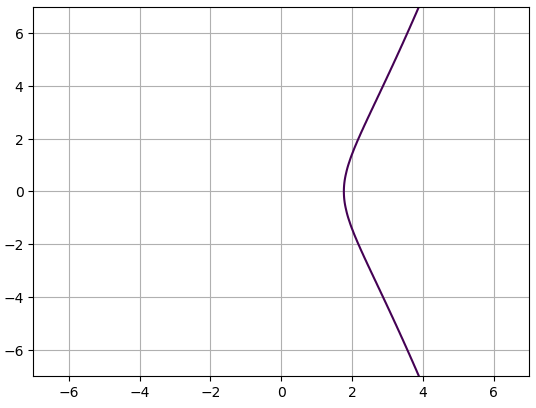
\includegraphics[width=\textwidth, valign=c]{ec_liscia_1.png}
        \caption{$E_{(-2, -2)}$}
    \end{minipage}
    \hfill
    \begin{minipage}[t]{0.45\textwidth}
        \centering
        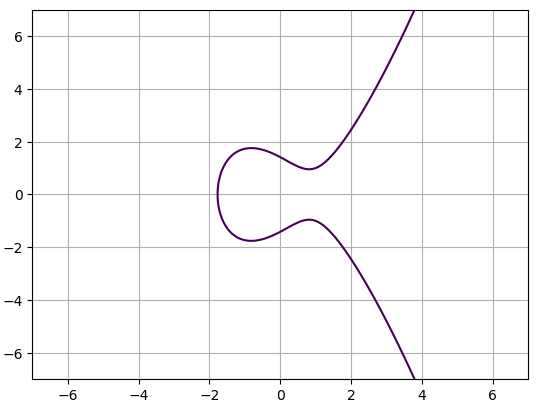
\includegraphics[width=\textwidth, valign=c]{ec_liscia_2.png}
        \caption{$E_{(-2, 2)}$}
    \end{minipage}\par
    \vskip\floatsep
    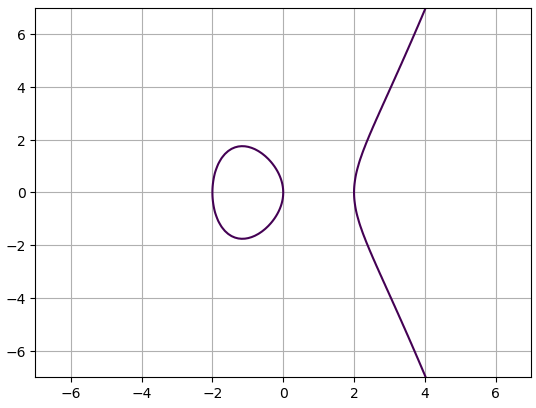
\includegraphics[width=0.45\textwidth]{ec_liscia_3.png}
    \caption{$E_{(-4, 0)}$}
\end{figure}

\newpage
\subsection{Curve Elittiche non Smooth}

\begin{figure}[h]
    \centering
    \begin{minipage}[t]{0.45\textwidth}
        \centering
        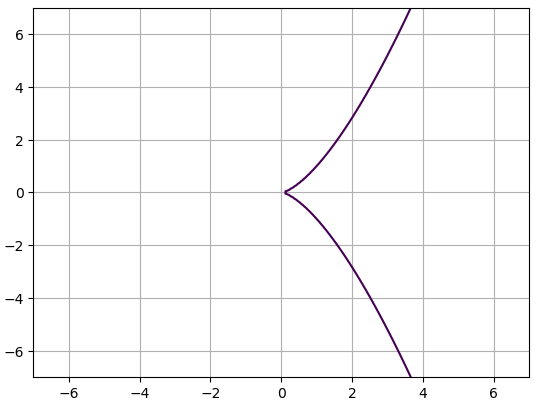
\includegraphics[width=\textwidth, valign=c]{ec_nonliscia_1.png}
        \caption{$E_{(0, 0)}$}
    \end{minipage}
    \hfill
    \begin{minipage}[t]{0.45\textwidth}
        \centering
        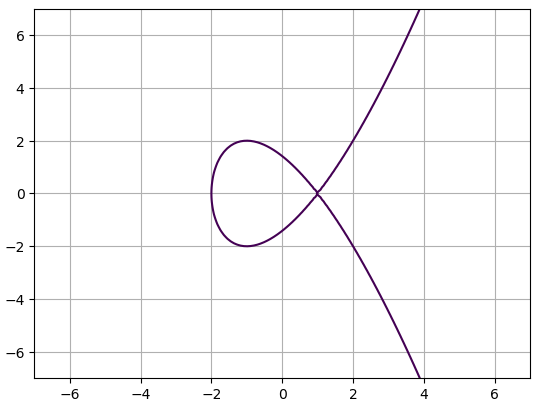
\includegraphics[width=\textwidth, valign=c]{ec_nonliscia_2.png}
        \caption{$E_{(-3, 2)}$}
    \end{minipage}
\end{figure}

\section{Operazioni Geometriche su una Curva}
\textbf{Intersezioni con una retta}: definiamo \textit{R} una retta di equazione $y = mx + q$ e una curva \textit{E} di equazione $y^2 = x^3 + ax + b$, avremo quindi le coordinate \textit{x} di intersezione tra \textit{R} e \textit{E} ($E \cup R$) definite implicitamente dagli zeri di $E(x, y) = y^2 - x^3 - ax - b$.
\begin{center}
    \begin{math}
        \begin{aligned}
            (mx + q) ^ 2 &=& x^3 + ax + b \\
            mx^2 + q^2 + 2mxq &=& x^3 + ax + b \\
            x^3 + ax + b - mx^2 - q^2 - 2mxq &=& 0 \\
            E(x, y) &=& x^3 - mx^2 - (a - 2mq) \cdot x - q^2
        \end{aligned}
    \end{math}
\end{center}
Si tratta di un polinomio \textbf{cubico} e sappiamo che, nel campo reale, esso deve avere \textbf{uno} o \textbf{tre zeri reali} (se ne ha uno solo, gli altri due zeri sono \textbf{complessi coniugati}). \\
Andando a studiare i casi particolari avremo:
\begin{center}
    \begin{math}
        E(x, y) =
        \begin{cases}
            x^3 + ax + b - q^2 \qquad m = 0 \\
            y^2 - c^3 - ac - b \qquad R: x = c 
        \end{cases}
    \end{math}
\end{center}
Su un \textbf{campo finito \textit{F}} non è assolutamente detto che un'equazione $P(x) = 0$, dove \textit{P} è un polinomio a coefficienti in \textit{F} di \textbf{grado dispari}, abbia almeno una soluzione in \textit{F}. È importante notare che nel caso in cui $F = \mathbb{Z}_p$ ha due zeri in \textit{F}, allora anche il terzo zero è in \textit{F}, tenendo presenti le molteplicità degli zero. Nel caso in cui, invece il polinomio a grado 2, ovvero è una \textbf{retta verticale} che incrocia la curva in \textbf{due punti} sarà necessario considerare un ulteriore punto di intersezione, che apparterrà ad un'estensione di F (reale o finito).

\begin{center}
    \textbf{\textit{m = 0}} $\Rightarrow$ \textbf{rette orizzontali}
    \begin{figure}[h]
        \centering
        \begin{minipage}[t]{0.45\textwidth}
            \centering
            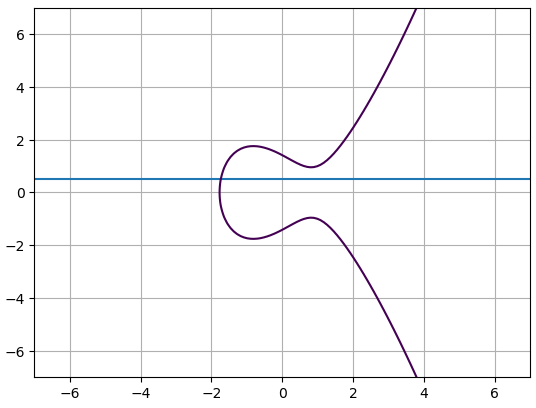
\includegraphics[width=\textwidth, valign=c]{m0_p1.png}
            \caption{$E_{(-2, 2)} \cup q = 0.5$}
        \end{minipage}
        \hfill
        \begin{minipage}[t]{0.45\textwidth}
            \centering
            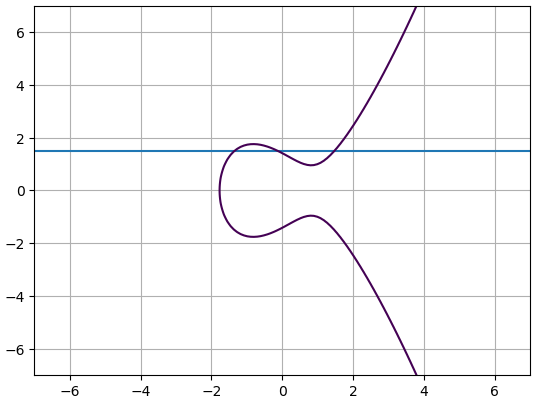
\includegraphics[width=\textwidth, valign=c]{m0_p3_1.png}
            \caption{$E_{(-2, 2)} \cup q = 1.5$}
        \end{minipage}\par
        \vskip\floatsep
        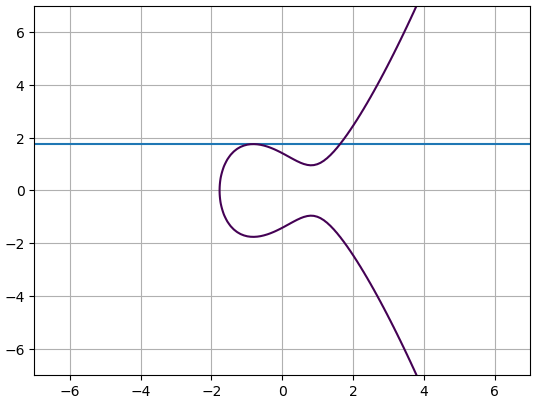
\includegraphics[width=0.45\textwidth]{m0_p3_2.png}
        \caption{$E_{(-2, 2)} \cup q = 1.7427$}
    \end{figure}
\end{center}
\begin{itemize}
    \item Nella \textit{Figura 6.6} abbiamo che la retta interseca una sola volta la curva.
    \item Nella \textit{Figura 6.7} abbiamo che la retta interseca la curva in tre punti, tutti con molteplicità \textit{1}.
    \item Nella \textit{Figura 6.8} abbiamo che la retta interseca 2 volte la curva, il primo punto altro non è che il punto di intersezione tra la curva e la tangente della curva in quel punto, che quindi avrà molteplicità \textit{2} e l'altro invece appartiene alla curva e quindi ha molteplicità \textit{1}
\end{itemize}

\begin{center}
    {\textbf{\textit{m = $\infty$}} $\Rightarrow$ \textbf{rette verticali}
    \begin{figure}[h]
        \centering
        \begin{minipage}[t]{0.45\textwidth}
            \centering
            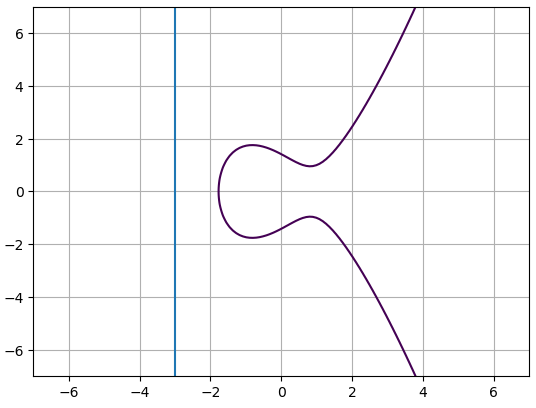
\includegraphics[width=\textwidth, valign=c]{m_inf_p0.png}
            \caption{$E_{(-2, 2)} \cup m = \infty, q = -3$}
        \end{minipage}
        \hfill
        \begin{minipage}[t]{0.45\textwidth}
            \centering
            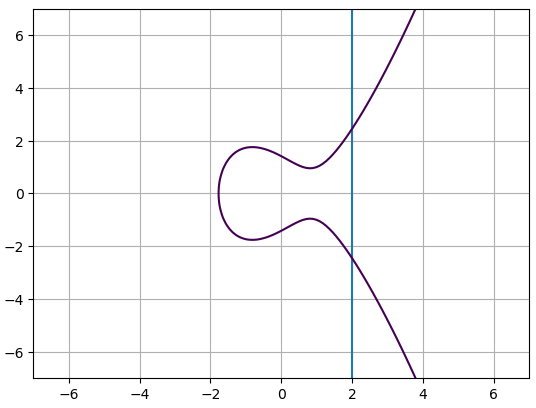
\includegraphics[width=\textwidth, valign=c]{m_inf_p2_1.png}
            \caption{$E_{(-2, 2)} \cup m = \infty, q = 2$}
        \end{minipage}\par
        \vskip\floatsep
        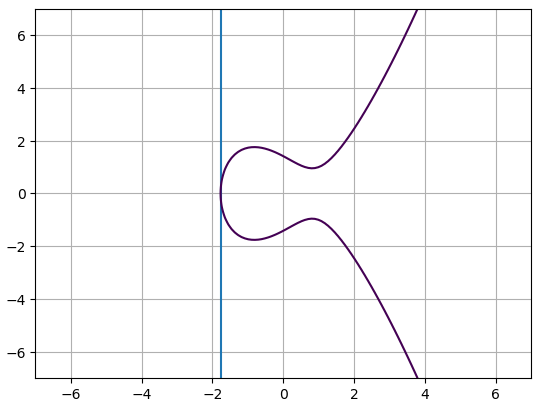
\includegraphics[width=0.45\textwidth]{m_inf_p2_2.png}
        \caption{$E_{(-2, 2)} \cup m = \infty, q = -1.76$}
    \end{figure}}
\end{center}
\begin{itemize}
    \item Nella \textit{Figura 6.9} abbiamo che la retta non interseca la curva.
    \item Nella \textit{Figura 6.10} abbiamo che la retta interseca la curva in due punti, tutti con molteplicità \textit{1}.
    \item Nella \textit{Figura 6.11} abbiamo che la retta interseca la curva come tangente di essa, quindi il punto avrà molteplicità \textit{2}.
\end{itemize}

\newpage
\begin{center}
    \textbf{\textit{m > 0, finito}} $\Rightarrow$ \textbf{rette oblique}
    \begin{figure}[h]
        \centering
        \begin{minipage}[t]{0.45\textwidth}
            \centering
            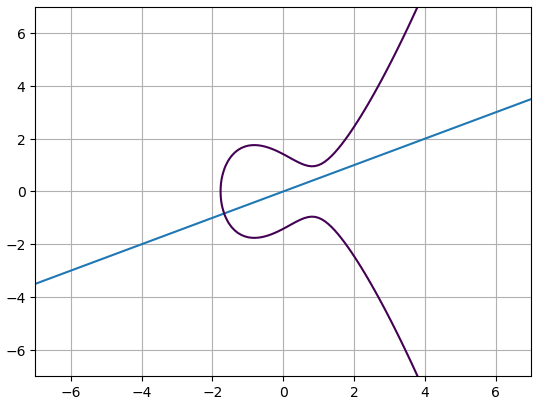
\includegraphics[width=\textwidth, valign=c]{m_p1.png}
            \caption{$E_{(-2, 2)} \cup m = 4$}
        \end{minipage}
        \hfill
        \begin{minipage}[t]{0.45\textwidth}
            \centering
            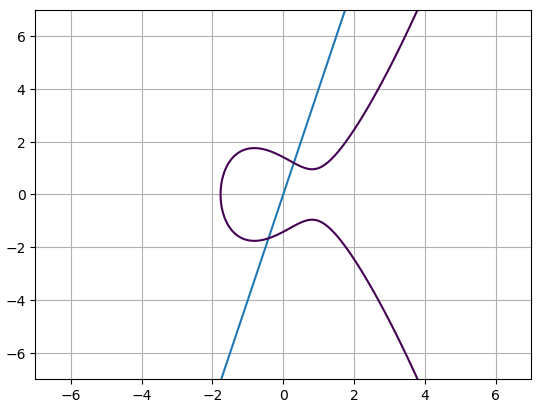
\includegraphics[width=\textwidth, valign=c]{m_p3_1.png}
            \caption{$E_{(-2, 2)} \cup m = 0.5$}
        \end{minipage}
        \begin{minipage}[t]{0.45\textwidth}
            \centering
            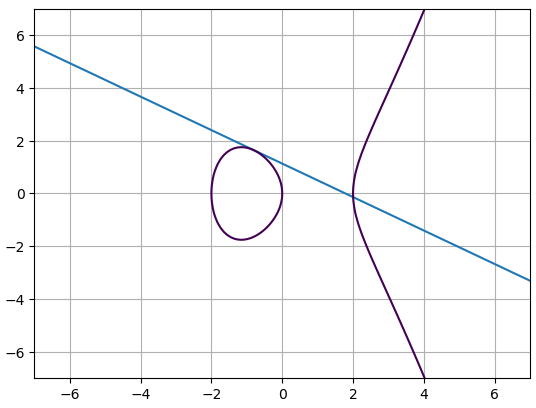
\includegraphics[width=\textwidth, valign=c]{m_p3_2.png}
            \caption{$E_{(-2, 2)} \cup m = -0.741, q = 1.416$}
        \end{minipage}
        \hfill
        \begin{minipage}[t]{0.45\textwidth}
            \centering
            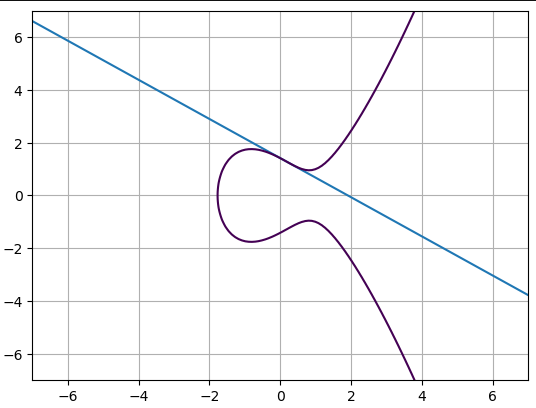
\includegraphics[width=\textwidth, valign=c]{m_p3_3.png}
            \caption{$E_{(-2, 2)} \cup m = -0.634, q = 1.132$}
        \end{minipage}
    \end{figure}
\end{center}
\begin{itemize}
    \item Nella \textit{Figura 6.12} avremo che la retta interseca la curva in un unico punto.
    \item Nella \textit{Figura 6.13} in questo caso avremo che la retta interseca, visivamente, la curva in soli due punti, entrmabi con molteplicità \textit{1}, ma sappiamo che siccome la curva \textit{E}, al crescere di \textit{x}, si comporta come $x^{\frac{3}{2}}$, quindi con velocità \textit{superlineare}, sappiamo che sarà presente un altro punto di intersezione con molteplicità \textit{1}.
    \item Nella \textit{Figura 6.14}: abbiamo che la retta interseca 2 volte la curva, il primo punto altro non è che il punto di intersezione tra la curva e la tangente della curva in quel punto, che quindi avrà molteplicità \textit{2} e l'altro invece appartiene alla curva e quindi ha molteplicità \textit{1}
    \item Nella \textit{Figura 6.15}: in questo caso la retta interseca la curva in un unico punto, che però essendo un punto di \textbf{flesso} della curva ha molteplicità \textit{3}.
\end{itemize}
Abbiamo definito che ai fini \textbf{crittografici} i casi di interesse sono quelli in cui sono presenti \textbf{3 punti di intersezione}. È infatti possibile definire un \textbf{gruppo} costituito proprio dai punti sulla curva. Nel caso di rette \textbf{verticali} ovvero con $m = \infty$ sono presente unicamente due punti di intersezione sulla curva. Detta in maniera discorsiva, vorremmo che quando sono presenti due intersezioni ce ne fosse \textbf{sempre} una terza, mentre invece se non ci sono intersezioni o ce n'è una sola \textbf{non sono rilevanti}. \\
La soluzione più semplice è quella di considerare un punto ``extra'', che indicheremo con $\mathcal{O}$, detto anche \textbf{Punto all'Infinito}. Il punto viene aggiunto ad \textit{F} ed è inteso far parte di qualsiasi curva \textit{E} su \textit{F}. Come vedremo $\mathcal{O}$ fungerà da \textbf{elemento neutro} dell'operazione di gruppo. \\
Proprietà di $\mathcal{O}$ :
\begin{itemize}
    \item qualsiasi \textbf{retta verticale} interseca \textit{E} in $\mathcal{O}$ con molteplicità \textit{1}, ne consegue che se \textit{R} ha già due intersezioni con \textit{E} il \textbf{punto all'infinito} costituirà il terzo punto di intersezione.
    \item nessuna retta con di equazione $y = mx + q$ con $m > 0$ finito interseca il punto $\mathcal{O}$.
    \item nel punto $\mathcal{O}$ la curva ha tangente \textit{t}. Si suppone che che \textit{t} abbia come unica intersezione con la curva proprio il punto $\mathcal{O}$ con molteplicità \textit{3}.
    \item $\mathcal{O}$ coincide con il suo opposto $-\mathcal{O}$.
    \item con l'introduzione del punto all'infinito, \textit{E} gode della seguente proprietà: \textbf{Sia \textit{R} una retta definita in \textit{F}, se \textit{R} ha due punti di intersezione in \textit{F} con la curva \textit{E}, allora ha anche un terzo punto di intersezione in \textit{F}}.
\end{itemize}

\newpage
\textbf{Addizione su Curva Elittica} \\
La somma di due punti $A, B \in E$ è definita come $A + B = -C$ ovvero la somma di \textit{A} e \textit{B} è il punto simmetrico al terzo punto di intersezione che risolve il sistema:
\begin{center}
    \begin{math}
        \begin{cases}
            y^2 = x^3 + ax + b \\
            y = mx + q
        \end{cases}
    \end{math}
\end{center}

\begin{figure}[h]
    \centering
    \begin{minipage}[t]{0.45\textwidth}
        \centering
        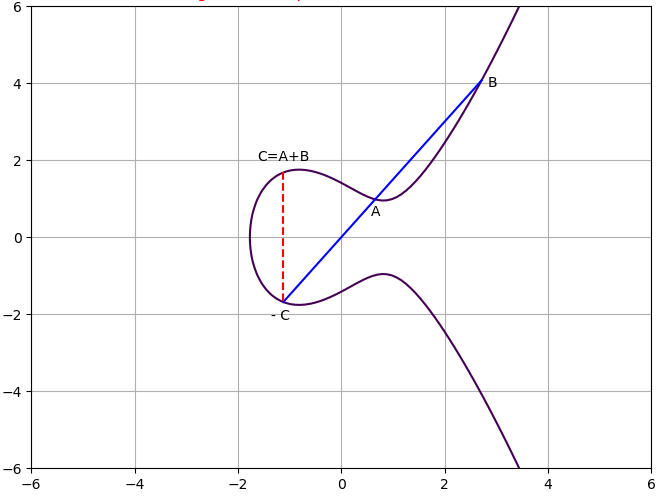
\includegraphics[width=\textwidth, valign=c]{sum_a_b_ec_p3_1.png}
        \caption{Caso generale}
    \end{minipage}
    \hfill
    \begin{minipage}[t]{0.45\textwidth}
        \centering
        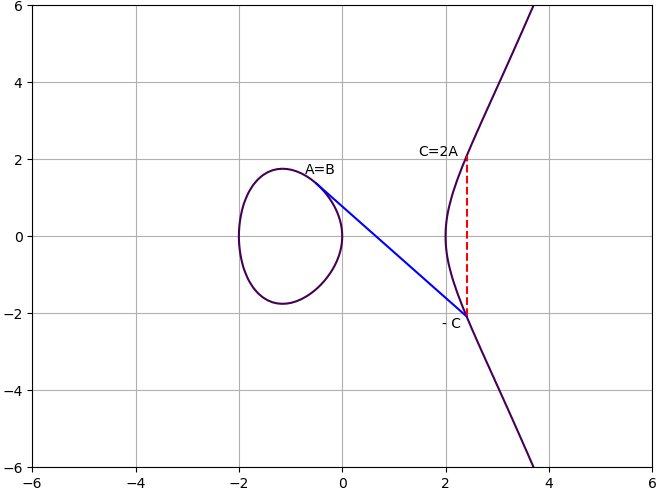
\includegraphics[width=\textwidth, valign=c]{sum_a_b_ec_p2_2.png}
        \caption{Caso di punti coincidenti}
    \end{minipage}
    \begin{minipage}[t]{0.45\textwidth}
        \centering
        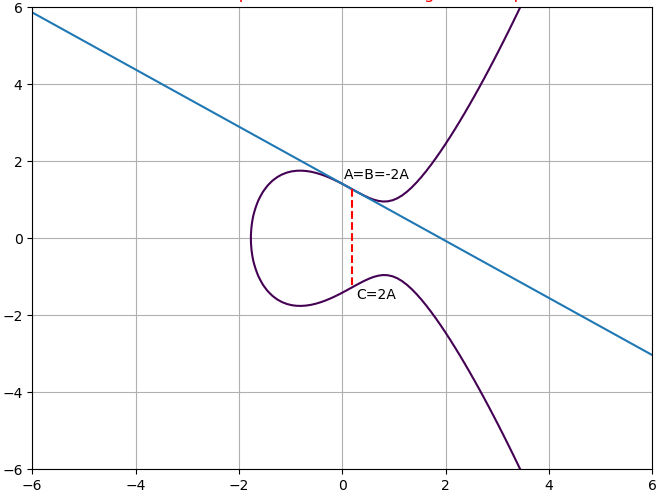
\includegraphics[width=\textwidth, valign=c]{sum_a_b_ec_p1_3.png}
        \caption{Caso di punto con flesso}
    \end{minipage}
    \hfill
    \begin{minipage}[t]{0.45\textwidth}
        \centering
        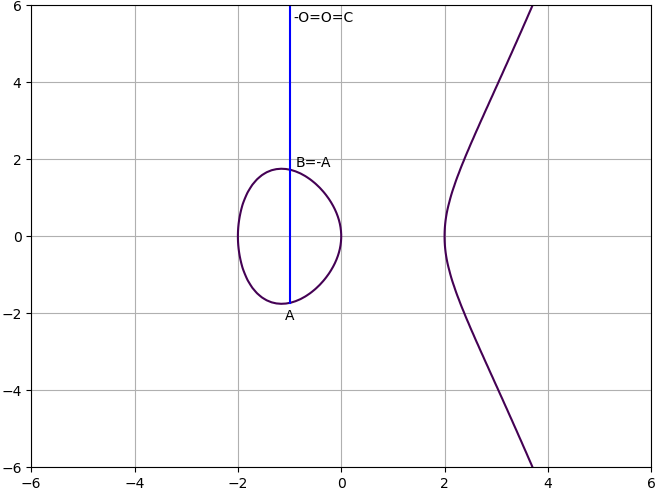
\includegraphics[width=\textwidth, valign=c]{sum_a_b_ec_p2_1.png}
        \caption{Caso retta verticale}
    \end{minipage}
\end{figure}
I punti sulla curva elittica con operazione di addizione appena definita formano un gruppo \textbf{abelliano}, ovvero un gruppo dove è definita la proprietà \textbf{commutativa}. Il gruppo generato mantiene anche la proprietà di \textbf{associazione} rispetto alla somma di punti. 
\begin{enumerate}
    \item \textbf{Chiusura}, in forza anche dell'introduzione del punto $\mathcal{O}$.
    \begin{itemize}
        \item i casi in cui i due punti sono diversi da $\mathcal{O}$ sono definiti geometricamente nelle \textit{Figure 6.16, 6.17, 6.18} in tutti i casi $A + B$ è ancora un punto della curva (eventualmente $\mathcal{O}$).
        \item $\mathcal{O} + \mathcal{O} = \mathcal{O}$, infatti per la proprietà del \textbf{punto all'infinito} sappiamo che $\mathcal{O}$ ha molteplicità 3 e che quindi la terza intersezione è $\mathcal{O}$, ma anche il suo \textbf{simmetrico}.
        \item $A + \mathcal{O} = A$.
    \end{itemize}
    \item $\mathcal{O}$ è l'elemento \textbf{neutro}: $A + \mathcal{O} = \mathcal{O} + A = A$
    \item ogni elemento \textit{A} ha un opposto, precisamente il punto di simmetria sulla curva \textit{-A}, infatti $A + (-A) = \mathcal{O}$.
    \item la proprietà \textbf{associativa} è verificata.
    \item la proprietà \textbf{commutativa} è verificabile geometricamente in quanto la retta che passa per due punti è individuabile indipendentemente dall'ordine dei punti.
\end{enumerate}
\   \\
\textbf{Caso A $\neq$ B} \\
Noti i punti $A(x_a, y_a) \text{ e } B(x_b, y_b)$ che sono soluzioni per il sistema:
\begin{center}
    \begin{math}
        \begin{cases}
            y^2 = x^3 + ax + b \\
            y = mx + q
        \end{cases}
        \Rightarrow R = 
        \begin{cases}
            y = y_a = y_b \qquad \text{ se } m = 0 \\
            y = (\frac{y_b - y_a}{x_b - x_a})x + (y_a - (\frac{y_b - y_a}{x_b - x_a}) \cdot x_a)
        \end{cases}
    \end{math}
\end{center}
$$\Rightarrow (mx + q)^2 = x^3 + ax + b \Rightarrow x^3 - mx^2 + (a - 2mq)x + b - q^2 = 0$$
Siccome due soluzione le conosciamo già e sappiamo che sono $A(x_a, y_a) \text{ e } B(x_b, y_b)$, possiamo visualizzare le \textit{x} del polinomio di terzo grado come: $(x - x_a)(x - x_b)(x - x_{\overline{c}}) = 0$ a noi interessa trovare il punto $-C(x_{\overline{c}}, y_{\overline{c}})$ che intersechi la curva \textit{E} appartente alla retta descritta da \textit{A} e \textit{B}.
\begin{center}
    \begin{math}
        \begin{aligned}
            (x - x_a)(x - x_b)(x - x_c) &= 0 \\
            x^3 - mx^2 + (a - 2mq)x + b - q^2 &= 0 \\
            (x - x_a)(x - x_b)(x - x_c) &= x^3 - mx^2 + (a - 2mq)x + b - q^2 \\
            x^3 + x^2 \cdot (- x_a - x_b - x_c) + x \cdot (x_a x_b + x_a x_c + x_b x_c) + x_a x_b x_c &= x^3 - mx^2 + (a - 2mq)x + b - q^2
        \end{aligned}
    \end{math}
\end{center}
Ugualiando i coefficienti di grado \textit{2} avremo: $-m^2 = - x_a - x_b - x_c$ e quindi potremo trovare la coordianta del punto $-C(x_{\overline{c}}, y_{\overline{c}}) = (m^2 - x_a - x_b, m \cdot x_{\overline{c}} + q)$. Il punto somma $C = A + B = -(-C)$ e siccome abbiamo detto che la \textbf{EC} è simmetrica rispetto all'asse delle \textit{x} avremo che $x_{\overline{c}} = x_c$ e $y_{\overline{c}} = -y_c$ andando così a descrivere il punto $C(x_c, y_c)$.
\\ \newline
\textbf{Caso A = B} \\
Quando i due punti coincidono è necessario calcolare il \textbf{coefficente angolare \textit{m}} della retta $R_A$ tangente alla curva per il punto \textit{A}. Anche se la curva non è definita in maniera esplicita è possibile rappresentarla come l'unione dei graifici di due funzioni, più precisamente:
$$y_1(x) = \sqrt{x^3 + ax + b} \;\;\; \cup y_2(x) = - \sqrt{x^3 + ax + b}$$
Dobbiamo quindi calcolare la derivata $\frac{d}{dx}y_1(x')$ e $\frac{d}{dx}y_2(x')$ dove $(x', y')$ è un punto definito sulla curva $y_1 \text{ se } y' \geq 0$, quindi vale $y_1(x') = y'$ mentre invece è definito sulla curva $y_2 \text{ se } y' \leq 0$, quindi vale $y_2(x') = y'$ possiamo calcolare i coefficienti delle rette tangenti:
\begin{center}
    \begin{math}
        \begin{aligned}
        \frac{d}{dx}y_1(x') &= \frac{3x'^2 + a}{2\sqrt{x'^3 + ax' + b}} = \frac{3x'^2 + a}{2y_1(x')} =& \frac{3x'^2 + a}{2y'} \\
        \frac{d}{dx}y_2(x') &= - \frac{3x'^2 + a}{2\sqrt{x'^3 + ax' + b}} = - \frac{3x'^2 + a}{2(- y_2(x'))} = - \frac{3x'^2 + a}{-2y'} =& \frac{3x'^2 + a}{2y'}
        \end{aligned}
    \end{math}
\end{center}
Avremo quindi che il calcolo del \textbf{coefficente angolare} è \textcolor{blue}{$m = \frac{3x'^2 + a}{2y'}$}. \\
Pseudo-codice per il calcolo di \textbf{C = A + B}:
\begin{lstlisting}[label=lst:rho-polland, basicstyle=\small, mathescape=true]
def sumPointOnEC(A: point, B: point) -> point:
    if A = = $\mathcal{O}$: return B
    if B = = $\mathcal{O}$: return A
    if B = = -A: return $\mathcal{O}$

    if $A \neq B$: m = $\frac{y_b - y_a}{x_b - x_a}$
    if $A == B$: m =  $\frac{3x_a^2 + a}{2y_a}$
        
    # C(x, y)
    return point($m^2 - x_a - x_b$, $- (mx_c + q)$)
\end{lstlisting}

\section{Curve in $\mathbb{Z}_p$}
Indicheremo una curva elittica a coefficienti \textit{a} e \textit{b}, definita sul campo $\mathbb{Z}_p$, usando la notazione $E_{a,b}(\mathbb{Z}_p)$.
\begin{figure}[h]
    \centering
    \begin{minipage}[t]{0.45\textwidth}
        \centering
        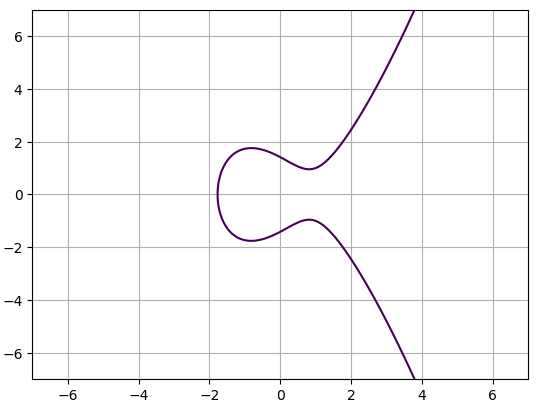
\includegraphics[width=\textwidth, valign=c]{ec_liscia_2.png}
        \caption{$E_{(-2, -2)}$}
    \end{minipage}
    \hfill
    \begin{minipage}[t]{0.45\textwidth}
        \centering
        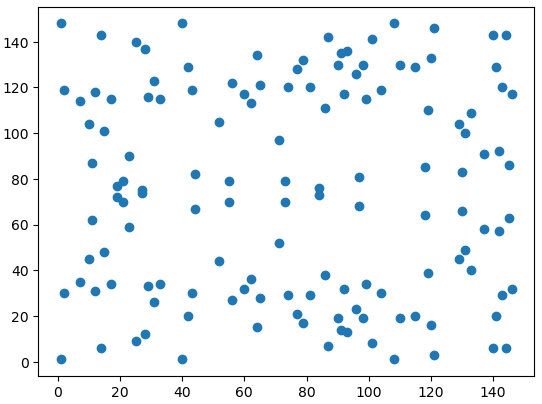
\includegraphics[width=\textwidth, valign=c]{ec_liscia_2_zp.png}
        \caption{$E_{-2, 2}(\mathbb{Z}_{149})$}
    \end{minipage}
\end{figure}
\   \\
Anche se, come possiamo notare, la geometria qui non ci può aiutare, i risultati algebrici rimangono ancora validi. Se un'equazione cubica (a coefficienti in $\mathbb{Z}_p$) ha due radici in $\mathbb{Z}_p$, allora ha anche la terza radice in $\mathbb{Z}_p$. Questo consenti di definire l'operazione di addizione come nel caso reale. Analogamente a quanto fatto per il gruppo $\mathbb{Z}_p^*$, possiamo definire dei \textbf{sottogruppi ciclici} dei punti $S_{E_{a,b}}(\mathbb{Z}_p)$. Il sottogruppo generato da un punto $g(x_g, y_g)$ è definito nel seguente modo:
\begin{center}
    \begin{math}
        S_{E_{a,b}(\mathbb{Z}_p)}(g)=\{a\in E_{a,b}(\mathbb{Z}_p)|\exists k\geq0, a = k\cdot g = \underbrace{g+g+\ldots+g}_{k-1\ \mathrm{somme}}\}
    \end{math}
\end{center}
L'operazione $k\cdot g$, dove $k$ è un intero non negativo e $g$ è un punto sulla curva, è detta \textbf{\textit{moltiplicazione scalare}}. Normalmente il gruppo dei punti sulla curva \textbf{non è ciclico}, per esso vale il teorema di \textbf{\textit{lagrange}}, ma non quello fondamentale dei gruppi ciclici.
\\ \newline
\textbf{Logaritmo Discreto su Curva Elittica} \\
Se \textit{g} è un punto sulla curva $S_{E_{a,b}(\mathbb{Z}_p)}$ che genera l'intero gruppo (quindi \textit{g} è una \textbf{radice primitiva} di $S_{E_{a,b}(\mathbb{Z}_p)}$), allora per ogni altro punto $z \in S_{E_{a,b}(\mathbb{Z}_p)} \rightarrow \exists k \geq 0 \; | \; z = k \cdot g$. Il minimo intero \textit{k} che soddisfa questa ugualianza è il \textbf{logaritmo a base \textit{g} di \textit{z}} rappresentabile nella forma $k = \log_{g}{z}$. Da un punto di vista computazionale, dati \textit{k} e \textit{g} è facile trovare il valore di \textit{z}, infatti l'algoritmo segue lo stesso schema dell'esponenziale modulare, ovvero il \textbf{\textit{Recursive Doubling}}. Il calcolo di \textit{z} parte dalla rappresentazione binaria di \textit{k} accumulando le quantità solo in corrispondenza degli \textit{1} della rappresentazione binaria di \textit{k}, il calcolo inverso, ovvero dati \textit{g} e \textit{z} trovare \textit{k} è invece \textbf{computazionalemente difficile} e non sono noti algoritmi con costo polinomiale. \\
Date le proprietà presenti del gruppo $E_{a,b}(\mathbb{Z}_p)$ è quindi facile immaginare del perché le \textbf{EC} abbiamo suscitato un tale interesse nell'ambito della crittografia. È però interessante osservare la questione dei \textbf{numeri di punti sulla curva}, infatti questo è l'\textbf{ordine} del nostro gruppo $E_{a,b}(\mathbb{Z}_p)$, quando si lavorava su gruppo $\mathbb{Z}_p^*$ l'ordine veniva facilmente calcolato dalla quantità $p - 1$ e quindi si potevano prendere delle precauzioni per evitare che i sottogruppi di $\mathbb{Z}_p^*$ avessero un ordine molto piccolo, grazie al \textbf{teorema di Lagrange} e la diretta costruzione del primo del tipo $p = 2q + 1$ dove anche \textit{q} fosse un numero primo. In questo modo si poteva controllare l'ordine dei sottogruppi di $\mathbb{Z}_p^*$ e quindi tenerli controllati in modo da evitare che fossero fattori semplici di \textit{p} (concetto dei \textbf{safe prime}). Nel caso delle \textbf{EC} non abbiamo un ``teorema'' che ci possa guidare alla scelta dei parametri \textit{a, b, p} in modo da controllare le dimensioni del gruppo dei punti sulla curva. 
\\ \newline
\textbf{Numeri di Punti sulla Curva}: se \textit{p} è il modulo, il numero di punti su una curva può superare il valore di $2p + 1$ questo perché se $x^3 + ax + b \bmod p \neq 0$ è un residuo quadratico, allora al valore \textit{x} corrispondono due radici in \textit{p} e quindi \textbf{due punti sulla curva}. Tuttavia per raggiungere il limite $2p + 1$ è necessario che $x^3 + ax + b$ sia un residuo quadratico modulo $p \; \forall x \in \{0, 1, ..., p - 1\}$ è però ragionevole attendersi che circa metà dei valori siano residui quadrati e metà residui non-quadratici in questo modo il numero di punti torna ad essere circa \textit{p}. Il numero di punti su una curva viene rappresentato da: $\#E(a, b, p)$. \\
Il \textbf{\textit{Teorema di Hasse}} fornisce un \textit{bound} più preciso:
\begin{center}
    $|\#E(a, b, p) - (p + 1)| \leq 2\sqrt{p}$
\end{center}
Dal punto di vista algoritmico, il miglior risultato noto per determinare il numero ``esatto'' di punti è dovuto a \textbf{\textit{\href{http://www.numdam.org/item/JTNB_1995__7_1_219_0.pdf}{René Schoof}}} la cui versione non ottimizzata dell'algoritmo ha complessità $\mathcal{O}((\log{p})^8)$ va però tenuto presente che per ogni curva l'algoritmo va eseguito una sola volta. In generale è sconsigliato cercare delle \textbf{safe curves} in autonomia, esistono già dei database in cui vengono salvate curve ritenute sicure (https://safecurves.cr.yp.to/).
\chapter{Algoritmi di Crittografia su elittica}
I parametri pubblici in un protocollo basato su una curva elittica includono sempre i seguenti dati:
\begin{enumerate}
    \item la \textbf{curva}: e quindi tutti i paramentri che la caratteristicano, ovvero \textit{a}, \textit{b} (i parametri dell'equazione) e \textit{p} (il modulo) e il numero di \textbf{punti} sulla curva.
    \item un punto \textit{P} che è generatore di un \textbf{sottogruppo ciclico} del gruppo formato da tutti i punti della curva (possibilmente di ordine elevato).
    \item un secondo punto \textit{Q} formato da $Q = k \cdot P$, per un qualche intero \textit{k} che è il segreto della comunicazione. 
\end{enumerate}
È chiaro che il poter risalire a \textit{k} da parte di \textit{Eve} permette di violare il codice, tuttavia il risalire a \textit{k} dai parametri pubblici dell'algoritmo è definito \textbf{\textit{Elliptic Curve Discrete Logarithm Problem}} anche noto come \textbf{\textit{ECDLP}} ed è computazionalmente intrattabile. Tuttavia è possibile risalire ad una \textbf{collisione} per poter risalire a \textit{k} dati i valori pubblici dell'algoritmo, attraverso la combinazione lineare a coefficienti interi dei due punti \textit{P} e \textit{Q}. \\
In altri termini dobbiamo trovare due coppie di numeri $\alpha_p, \alpha_q \text{ e } \beta_p, \beta_q$ tali che valga l'equazione:
\begin{center}
    \begin{math}
        \begin{aligned}
            \alpha_p \cdot P + \alpha_q \cdot Q &= \beta_p \cdot P + \beta_q \cdot Q \\
            \alpha_p \cdot P + k \cdot \alpha_q \cdot P &= \beta_p \cdot P + k \cdot \beta_q \cdot P \; || \; \Leftarrow Q = k \cdot P \\
            (\alpha_p + k \cdot \alpha_q)P &= (\beta_p + k \cdot \beta_q)Q
        \end{aligned}
    \end{math}
\end{center}
Analizzando i passaggi: i valori che cerca \textit{Eve} devono essere tali che $\alpha_p + k \cdot \alpha_q \equiv 0 \bmod \#E$ e $\beta_p + k \cdot \beta_q \equiv 0 \bmod \#E$ la ragione va ricercata utilizzando il \textbf{teorema di Lagrange}, infatti se i coefficenti sono congrui modulo il numero di punti, saranno congrui anche all'ordine del sottogruppo generato da \textit{P} in quanto, un gruppo che ha ordine \textit{k} avrà come ordine dei sottogruppi dei \textbf{divisori} di \textit{k}, se dunque quale la congruenza:
\begin{center}
    \begin{math}
        \begin{aligned}
            \alpha_p + k \cdot \alpha_q &\equiv 0 \bmod \#E \\
            \beta_p + k \cdot \beta_q &\equiv 0 \bmod \#E \\
            \alpha_p + k \cdot \alpha_q &\equiv \beta_p + k \cdot \beta_q \bmod \#E \\
            \alpha_p + k \cdot \alpha_q - \beta_p - k \cdot \beta_q &\equiv 0 \bmod \#E \\
            \alpha_p - \beta_p - k \cdot (\beta_q - \alpha_q) &\equiv 0 \bmod \#E \\
            \alpha_p - \beta_p &\equiv k \cdot (\beta_q - \alpha_q) \bmod \#E \\
        \end{aligned}
    \end{math}
\end{center}
Ottenendo quindi:
$$
k = (\alpha_p - \beta_p) \cdot (\beta_q - \alpha_q)^{-1} \bmod \#E \iff gcd(\beta_q - \alpha_q, \#E) = 1
$$
Con un argomento riducibile all ``dimostrazione'' del \textbf{paradosso del compleanno} possiamo dire che il tempo atteso nel caso di numeri di \textit{n} bit è $\mathcal{O}(2^{\frac{n}{2}})$. \\
I \textbf{protocolli crittografici} più comunemente utilizzati, fra quelli che impiegano curve elittiche, riguardano lo \textbf{scambio di chiavi} e la \textbf{firma digitale}. È infatti possibile avere con le \textbf{EC} un grado di sicurezza (espresso in bit) di $\frac{n}{2}$, con chiavi di \textit{n} bit e dunque $n = 256$ è tipicamente una lunghezza sufficente, quindi molto ``performante'', ma insufficiente per la \textbf{cifratura di messaggi}.

\newpage
\section{Elliptic Curve Diffie-Hellman}
\textbf{Descrizione del Protocollo}:
\begin{enumerate}
    \item \textit{Alice} e \textit{Bob} si accordano su una \textbf{curva elittica \textit{E}} ($E_{a,b}(\mathbb{Z}_p)$, $\#E$) e su un punto $P \in E_{a,b}(\mathbb{Z}_p)$.
    \item \textit{Alice} sceglie a caso un numero $k_a$ e determina il punto $A = k_a \cdot P$ che invia a \textit{Bob}.
    \item \textit{Bob} sceglie a caso un numero $k_b$ e determina il punto $B = k_b \cdot P$ che invia a \textit{Alice}.
    \item \textit{Alice} calcola $Z_a = k_a \cdot B$ con il punto \textit{B} ricevuto da \textit{Bob}
    \item \textit{Bob} calcola $Z_b = k_b \cdot A$ con il punto \textit{A} ricevuto da \textit{Alice}
    \item il punto $Z = Z_a = Z_b$ è il \textbf{segreto condiviso}, normalmente siccome \textit{Z} è nella forma $Z(x_z, y_z)$ viene scelta una delle due coordinate come segreto.
\end{enumerate}
La \textbf{correttezza del protocollo} è una l'applicazione della proprietà \textbf{associativa} all'interno di un gruppo $E_{a,b}(\mathbb{Z}_p)$:
$$Z_a = k_a \cdot B = k_a \cdot (k_b \cdot P) = k_b \cdot (k_a \cdot P) = k_b \cdot A = Z_b$$
Per quanto riguarda invece l'\textbf{efficienza} le operazioni più costose sono chiaramente i ``prodotti scalari'' per il calcolo della ``chiave pubblica'' e del segreto condiviso, dove però viene utilizzato l'algoritmo di \textbf{recursive doubling} e quindi possono essere considerati come addizioni di punti che è lineare alla lunghezza delle costanti segrete in gioco. Ogni addizione richiede, perciò, \textit{4} o \textit{5} moltiplicazioni nel campo $\mathbb{Z}_p^+$ oltre alle riduzioni in modulo. Il costo computazionale finale è perciò $\mathcal{O}(n^3)$ bit-operation.
\   \newpage
\textbf{Attacco basato sull'uso di una differente curva ``debole''} \\
La \textbf{condizione} per l'attacco è che \textit{Bob} non esegua un controllo sul punto che \textit{Alice} (\textit{Eve}) invia come \textbf{chiave pubblica}. \\
Definiamo $E_{a, b}(\mathbb{Z}_p)$ come curva scelta per la comunicazone, $\#E$ il numero di punti presenti sulla curva e un punto $P \in E_{a, b}(\mathbb{Z}_p)$. \textit{Bob} sceglie la propria \textbf{chiave privata} $k_b$ e calcola il punto $B = k_b \cdot P$ e lo invia ad \textit{Eve}. \\
\textit{Eve} sceglie un punto $A \in \overline{E}_{a, b}(\mathbb{Z}_p) \; | \; \mathcal{O} = p \cdot A$ dove avremo che $\#\overline{E} = p \cdot q$. Definiamo $\overline{E}_{a, b}(\mathbb{Z}_p)$ \textbf{``curva debole''} e $\#\overline{E}$ il numero di punti presenti sulla curva. A quel punto invia a \textit{Bob} la propria chiave pubblica: \textit{A}. \textit{Bob} calcolerà il \textbf{segreto condiviso} come $Z = k_b \cdot A$ e potrà iniziare a inviare messaggi cifrati ad \textit{Eve} come $C = Enc(M, hash(Z))$. Una volta ottenuto un messaggio cifrato \textit{Eve} non riuscirà a decifrarlo nella maniera \textit{standard}, però per costruzione potrà ricercare un punto $I \in S_{\overline{E}_{a, b}(\mathbb{Z}_p)}(A) \; | \; I = (A \cdot \mathcal{O}) \cdot m, \; m \in \{0, 1, ..., p - 1\}$ che permetterà di decifrare il messaggio $M = Dec(C, hash(I))$. A questo punto \textit{I} è quindi associato un valore \textit{m} che altro non è che il resto della divisione di $k_b$ ovvero il segreto di \textit{Bob} per uno dei due fattori di $\#\overline{E} \rightarrow p$. \\
Una volta ottenuto il primo dei due parametri per riuscire ad ottenere in maniera illegittima la \textbf{chiave segreta} di \textit{Bob}, \textit{Eve} dovrà ``fingere'' di aver sbagliato ad inviare la propria \textbf{chiave pubblica} attraverso tecniche di \textbf{\textit{Social Engineering}} e reinviare a \textit{Bob} un punto $A' \in \overline{E}_{a, b}(\mathbb{Z}_p) \; | \; \mathcal{O} = q \cdot A'$ dove \textit{q} è l'altro fattore di $\#\overline{E}$, \textit{Bob} ripeterà i passaggi fino a che \textit{Alice} non dovrà decifrare il nuovo messaggio inviato da \textit{Bob} utilizzando la formula: $I \in S_{\overline{E}_{a, b}(\mathbb{Z}_p)}(A) \; | \; I = (A \cdot \mathcal{O}) \cdot r, \; r \in \{0, 1, ..., q - 1\}$ una volta che avra ottenuto il punto \textit{I} che gli permetterà di decifrare il nuovo messaggio $M = Dec(C, hash(I))$ e quindi il corrispondente \textit{r} che altro non è che il resto della divisione intera di $k_b$ ovvero il segreto di \textit{Bob} per uno dei due fattori di $\#\overline{E} \rightarrow q$. \\
A questo punto \textit{Eve} può usare il \textbf{\textit{Chinese Remainder Theorem}} per costruire un $C \equiv k_b \bmod \#\overline{E}$
\begin{center}
        $C = q \cdot (q^{-1} \bmod p) \cdot m + p \cdot (p^{-1} \bmod q) \cdot r$ \\
        $k_b = C \bmod \#\overline{E}$
\end{center}
Vista la parte di \textbf{\textit{Social Engineering}} si cerca di contenere il numero di ``errori di invio della chiave'' il più basso possibile $\#\overline{E} = p \cdot q$, ma generalizzando, potrebbe essere $\#\overline{E} = p_1 \cdot p_2 \cdot p_h$ e bisognerebbe ingannare \textit{Bob} $h - 1$ volte.

\newpage
\section{Elliptic Curve - Digital Signature Algorithm}
\textbf{Descrizione del Protocollo}:
\begin{itemize}
    \item \textbf{Generazione delle Chiavi: \textit{Alice}}
    \begin{enumerate}
        \item fissa la curva $E_{a,b}(\mathbb{Z}_p)$ e un punto base $P \in E_{a,b}(\mathbb{Z}_p)$.
        \item determinato un numero $N = \#E_{a,b}(\mathbb{Z}_p)$ di punti sulla curva genera a caso un elemento $a \in \mathbb{Z}_p^+$ che conserva come \textbf{chiave privata}.
        \item calcola $A = a \cdot P$ e rende noto ($E_{a,b}(\mathbb{Z}_p)$, \textit{A}) come chiave \textbf{chiave pubblica}.
    \end{enumerate}
    \item \textbf{Firma del Messaggio: \textit{Alice}}
    \begin{enumerate}
        \item applica una funzione \textbf{hash} (pubblicamente nota) al messaggio \textit{M} da firmare, generando $h = hash(M) \bmod N$.
        \item sceglie a caso un numero $k \; | \; 0 < k < N \land gcd(k, N) = 1$ e calcola il punto $Q = k \cdot P$ sulla curva, $Q(x_q, y_q)$.
        \item Pone $r = Q_x \bmod N$ e $s = k^{-1} \cdot (h + r \cdot a) \bmod N$
        \item invia la $(M, (r, s))$.
    \end{enumerate}
    \item \textbf{Verifica della Firma: \textit{Bob}}
    \begin{enumerate}
        \item calcola l'\textbf{inverso moltiplicativo} di \textit{s} modulo \textit{N} cioè $w = s^{-1} \bmod N = k \cdot (h + r \cdot a)^{-1} \bmod N$.
        \item calcola i due prodotti
        \begin{center}
                $u = hash(M) \cdot w$ \\
                $v = r \cdot w$
        \end{center}
        \item determina il punto $R = (uP + vA) \bmod N$.
        \item accetta solo se $x_r = r$
    \end{enumerate}
\end{itemize}

\newpage
La \textbf{correttezza} dell'algoritmo è verificata in quanto (i calcoli sono modulo \textit{N}):
\begin{center}
    \begin{math}
        \begin{aligned}
            R &= u \cdot P + v \cdot A \\
            &= (h \cdot w) \cdot P + (r \cdot w) \cdot A \\
            &= h \cdot w \cdot P + r \cdot w(a \cdot P) \\
            &= w \cdot (h + r \cdot a) \cdot P \\
            &= (k \cdot (h + r \cdot a)^{-1}) \cdot (h + r \cdot a) \cdot P \\
            &= k \cdot P \\
            &= Q
        \end{aligned}
    \end{math}
\end{center}
Il valore casuale \textit{k} deve essere usato una sola volta, altrimenti è vulnerabile. Supponiamo che due messaggi $M_1 \text{ e } M_2$ con corrispondenti valori di hash $h_1 \text{ e } h_2$ vengano firmati con lo stesso valore \textit{k}. Questo porta ad avere anche lo stesso valore di \textit{r}, che è la coordinata \textit{x} (modulo \textit{N}) del punto $Q = k \cdot P$. \\
Indichiamo con $(r, s_1)$ e $(r, s_2)$ le due firme, l'attaccante può calcolare la quantità:
\begin{center}
    \begin{math}
        \begin{aligned}
            s_1 - s_2 &= k^{-1} \cdot (h_1 + r \cdot a) - k^{-1} \cdot (h_2 + r \cdot a) \\
            &= (h_1 + r \cdot a - h_2 - r \cdot a) \cdot k^{-1} \\
            &= (h_1 - h_2) \cdot k^{-1} \\
        \end{aligned}
    \end{math}
\end{center}
Riuscendo ad ottenere:
$$k = (s_1 - s_2)^{-1} \cdot (h_1 - h_2) \bmod N$$
Una volta ottenuto il \textit{k} per risalire alla chiave privata bisogna utilizzare una delle due firme:
\begin{center}
    \begin{math}
        \begin{aligned}
            s_1 &= k^{-1} \cdot (h_1 + r \cdot a) \\
            k \cdot s_1 &= (h_1 + r \cdot a) \\
            k \cdot s_1 - h_1 &= r \cdot a \\
            (k \cdot s_1 - h_1) \cdot r^{-1} &= a
        \end{aligned}
    \end{math}
\end{center}


% PAGINA VUOTA
%\clearpage\null\thispagestyle{empty}\clearpage
%\appendix
%\appendixpage
%\addappheadtotoc

%\clearpage\null\thispagestyle{empty}\clearpage


%\listoffigures


\begin{flushleft}
\bibliographystyle{plain}
\bibliography{sections/references} 
\end{flushleft}

\end{document}
